\defcitealias{ali_et_al2015}{A15}

\chapter{PAPER-64 Case Study}
\label{c.PSA64}


\section{Overview}
\label{sec:PSA64overview}

In the previous chapter we have discussed three overarching 21\,cm power spectrum themes --- signal loss, error estimation, 
and bias. Understanding the subtleties and trade-offs involved in each is necessary for an accurate and robust understanding of 
a power spectrum result. 

We now apply these lessons to data from the PAPER experiment in order to illustrate our revised analysis pipeline. We begin with a brief overview of PAPER's data processing steps prior to power spectrum estimation before delving into each theme in detail.

\subsection{Observations}

As described in Chapter \ref{sec:PAPER_intro}, PAPER is a dedicated 21\,cm experiment located in the Karoo Desert in South Africa. The PAPER-64 configuration consists of 64 dual-polarization drift-scan elements that are arranged in a grid layout (Figure \ref{fig:ant_layout}). While every unique baseline is used for calibration, only a subset of the baselines are used for the power spectrum analysis in \citetalias{ali_et_al2015} (the three baselines used are the $30$\,m East/West baselines and their off-diagonal companions where two antennas are in adjacent columns and neighboring rows) and only one baseline-type is used for the demonstrations in this chapter (only the $30$\,m East/West baselines).

PAPER-64 conducted nighttime observations from November 2012 to March 2013. Over the course of the season, LST-coverage varied slightly, with power spectrum analyses focusing on the ``cold patch" range from $\sim0$-$8$\,hours when the Galaxy is below the horizon. The PAPER correlator processes a 100-200\,MHz bandwidth that consists of 1024 channels, each of width 97.6\,kHz. Visibilities are integrated for 10.7\,s before being written to disk. 

PAPER's raw data is compressed by a factor of $\sim70$ through the use of RFI, delay, and delay-rate filters. More specifically, radio frequency interference is flagged at the $6\sigma$ level. Next, a low-pass delay filter is applied to all the data in order to filter out delays greater than the maximum delay allowed by the longest baseline in the array. Similarly, a low-pass fringe-rate, or delay-rate filter is applied to limit fringe-rates to allowable scales set by the array. Finally, the data is decimated to critical Nyquist sampling rates of 493\,kHz and 42.9\,s. For more details about PAPER's data acquisition and compression pipelines, we refer the reader to \citet{parsons_et_al2010} and \citetalias{ali_et_al2015}.

\begin{figure}
    \centering
    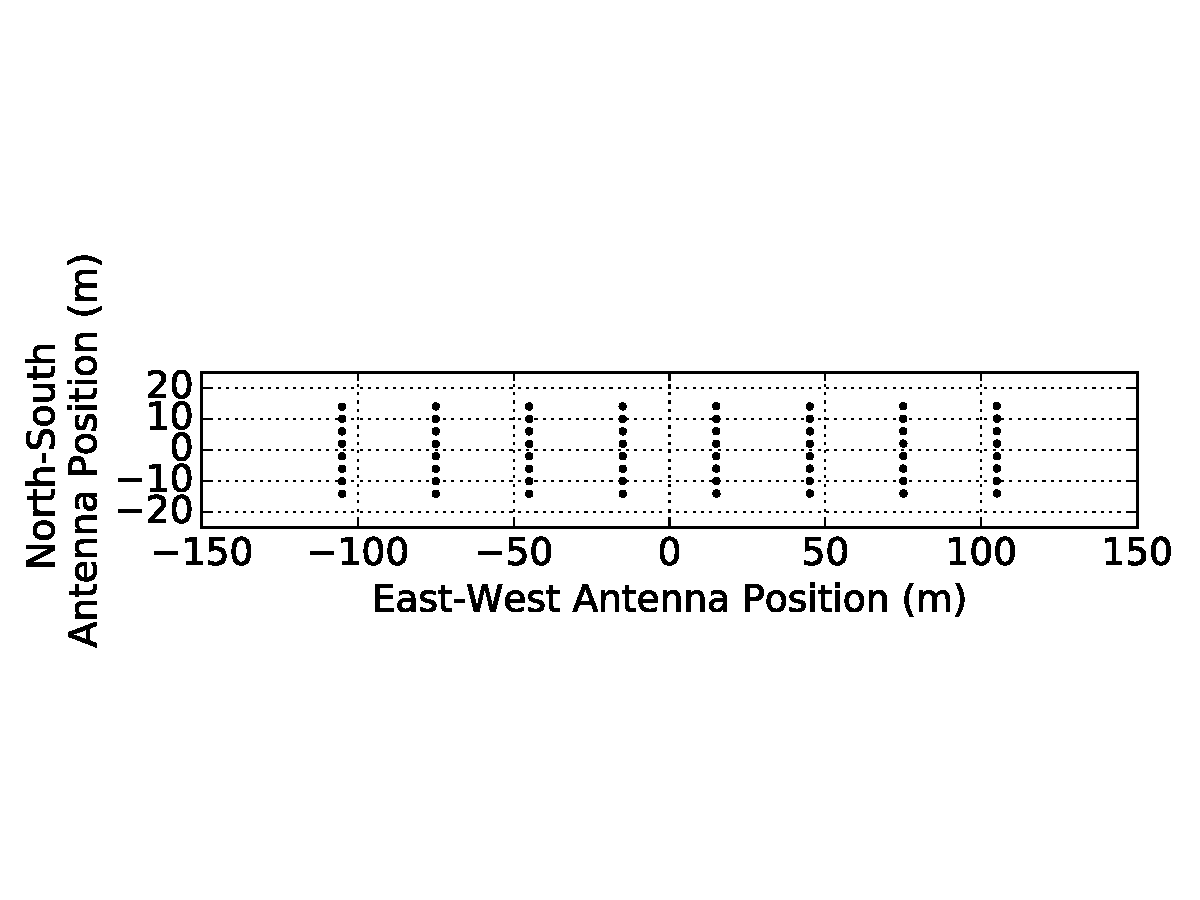
\includegraphics[trim={0cm 0cm 0cm 0cm},width=\columnwidth]{plots/ant_layout_aspect.pdf}
    \caption{The PAPER-64 antenna layout. We use only $10$ of the $30$ m East/West baselines for the analysis in this 
chapter (i.e., a subset of the shortest horizontal spacings).}
    \label{fig:ant_layout}
\end{figure}

\subsection{Data Processing}
\label{sec:PSA64_processing}

As described in Chapters \ref{sec:calibration_intro}, \ref{sec:fg_intro}, \ref{sec:frf_intro}, the primary post-processing steps of PAPER's compressed data is calibration, foreground-filtering, and fringe-rate filtering. We now give a brief overview of each, as applied to PAPER data.

We employ the package {\sc Omnical} for redundant calibration (\citealt{zheng_et_al2014}), which comprises of three steps. The first is {\tt FirstCal}, which uses all baseline redundancies to generate a static gain solution for each antenna that will unwrap any phase wrapping between two identical baselines. We perform {\tt FirstCal} because the next stage of {\sc Omnical} cannot tell the difference between a phase of $0$ and $2\pi$, for example. The second step is {\tt LogCal}, which takes the log of all the visibility equations (Equation \eqref{eq:gains}) and separates the real and imaginary components into two matrices. Coarse solutions are determined for both the antenna gains and ``model" visibilities (one for each baseline type) simultaneously. The final step of {\sc Omnical} is {\tt LinCal}, which applies small perturbations to the {\tt LogCal} solutions in an iterative fashion, honing in on the optimal solutions.
 
It is important to note that while {\sc Omnical} is powerful for ensuring array redundancy, it is not able to solve for $4$ calibration parameters - namely, the overall gain, phase, and tip/tilt of the array. For absolute calibration, we turn to a standard self-calibration routine which includes imaging Pictor A, Fornax A, and the Crab Nebula in order to fit for the overall phase solutions and the flux scale.

After calibration, we combine the XX and YY linear polarization data to form pseudo-Stokes I as defined as:

\begin{equation}
\label{eq:stokes}
V_{I} = \frac{1}{2}(V_{XX}+V_{YY})
\end{equation}
(\citealt{moore_et_al2013}).

Next, a delay-filter is used to filter out foregrounds contained inside the maximum delay set by each baseline. This is accomplished by de-convolving out our sampling function (which contains flags due to RFI) from our delay-domain visibilities using a CLEAN-like algorithm that restricts our clean components to inside the horizon limit, plus a 15\,ns buffer. The Fourier-transformed clean components are then subtracted from our visibilities. This filtering process is performed on a per-baseline, per-integration basis, and we achieve a brightness suppression of $\sim4$ orders of magnitude in our visibilities.

After delay-filtering, we perform a final round of RFI-removal by flagging visibilities that lie more than $3\sigma$ above the mean on a time, frequency, and baseline basis. Finally, we stack our data in LST into two datasets, alternating between even and odd Julian Dates to create an ``even" and ``odd" LST-binned dataset. A total of 124 days of data are included in the LST-binned dataset.

The final step before power spectrum estimation is fringe-rate filtering. The chosen filter (which is described in the next section) is applied on a per-baseline basis and weights the fringe-rate bins on the sky by the RMS of the primary beam at that same location. A smooth filter is constructed by fitting a Gaussian to the filter shape in the fringe-rate domain. Additionally, fringe-rates below 0.2\,mHz are zeroed out, effectively removing slowly-varying signals such as crosstalk. We then convolve our time-domain visibilities by the Fourier-transform of the fringe-rate filter to yield time-averaged visibilities that have gained another order of magnitude in sensitivity.

\subsection{Case Study Data}

For the case study presented in the rest of this chapter, we 
focus on a subset of the PAPER-64 data used in \citetalias{ali_et_al2015}, namely, on LST-binned, Stokes I estimated data \citep{moore_et_al2013} from PAPER's $30$ m East/West baselines (Figure 
\ref{fig:ant_layout}). Hence, all data processing steps are identical to those in \citetalias{ali_et_al2015} until after the LST-binning step in Figure 3 of \citetalias{ali_et_al2015}.

The previously best published 21\,cm upper limit result from \citetalias{ali_et_al2015} placed a $2\sigma$ upper limit 
on $\Delta^{2}(k)$, defined as

\begin{equation}
\Delta^{\textbf{2}}(k) = \frac{k^{3}}{2\pi^{2}}\,\hat{P}(k),
\end{equation}

\noindent of $(22.4$ mK$)^{2}$ in the range $0.15 < k < 0.5$\,$h$ Mpc$^{-1}$ at $z = 8.4$. The need to revise this limit stems mostly from previously under-estimated signal loss and under-estimated error bars, both of which we 
address in the following sections. 

For the analysis in this chapter, we use $8.1$ hours of LST, namely an RA range of $0.5$-$8.6$ hours (\citetalias{ali_et_al2015} uses a slightly longer RA 
range of $0$-$8.6$ hours; we found that some early LSTs were more severely foreground contaminated). We also use only $10$ baselines, a subset of the $51$ total East/West baselines used in \citetalias{ali_et_al2015}, in order to illustrate our revised methods. All power spectrum results are produced for a center frequency of 151\,MHz using a width of 10\,MHz ($20$ channels), identical to the analysis in \citetalias{ali_et_al2015}. In the case study in this chapter, we only use one baseline type instead of the three as in 
\citetalias{ali_et_al2015}, but Chapter \ref{c.PSA64_results} uses the full dataset presented in \citetalias{ali_et_al2015} to revise the result and place limits on the EoR at multiple redshifts (using a straightforward and not lossy approach to avoid many of the issues presented in this chapter).

The most significant changes from \citetalias{ali_et_al2015} occur in our revised power spectrum analysis, which is explained in the rest of this chapter, but we also note that the applied fringe-rate filter is also slightly different. In \citetalias{ali_et_al2015}, the 
applied filter was not equivalent to the optimal fringe-rate filter (which is designed to maximize power spectrum sensitivity). Instead, the optimal filter was degraded slightly by widening it in fringe-rate space. This was chosen in order to increase the number of independent 
modes and reduce signal loss associated with the quadratic estimator, though as we will explain in the next section, this signal loss was still under-estimated. With the development of a new, 
robust method for assessing signal loss, we choose to use the optimal filter in order to maximize sensitivity. This filter is 
computed for a fiducial 30\,m baseline at 150\,MHz, the center frequency in our band. The filter in both the fringe-rate 
domain and time domain is shown in Figure \ref{fig:frp}.

Finally, we emphasize that the discussion that follows is solely focused on signal loss associated with empirical covariance weighting. As mentioned in Chapter \ref{sec:SiglossOverview}, there are a number of steps in our analysis pipeline which could lead to loss, including gain calibration, delay filtering, and fringe-rate filtering, which have been investigated at various levels of detail in \citet{parsons_et_al2014} and \citetalias{ali_et_al2015} but are clearly the subject of future work. Here we only focus on the most significant source of loss we have identified and note that Chapter \ref{c.PSA64_results} and other future work will consider additional sources of signal loss and exercise increased caution in reporting results.

\begin{figure}
    \centering
    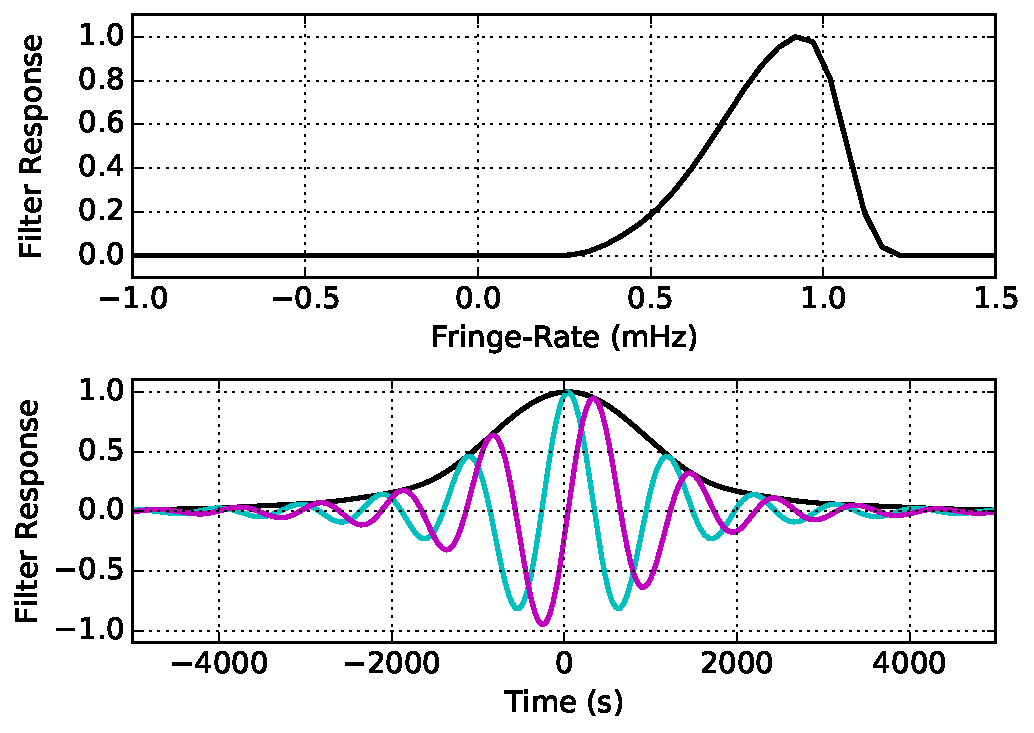
\includegraphics[width=0.6\textwidth]{plots/frp.pdf}
    \caption{Top: the normalized optimal power-spectrum sensitivity weighting in fringe-rate space for our fiducial baseline and 
Stokes I polarization beam. Bottom: the time domain convolution kernel corresponding to the top panel. Real and imaginary 
components are illustrated in cyan and magenta, respectively, with the absolute amplitude in black. The fringe-rate filter acts as 
an integration in time, increasing sensitivity but reducing the number of independent samples in the dataset.}
    \label{fig:frp}
\end{figure}

\section{Signal Loss}
\label{sec:CaseStudy}

We present our PAPER-64 signal loss investigation in three parts. We first give an overview of our signal injection framework which is used to estimate loss (Chapter \ref{sec:siglossmethod}). In this framework (and as in \citetalias{ali_et_al2015}), we inject simulated cosmological signals into our data and test the recovery of those signals (an approach also taken by \citet{masui_et_al2013}). As we will see, correlations between the injected signals and the data are significant complicating factors which were previously not taken into account. Next, we describe our methodology in practice and detail how we map our simulations into a posterior for the EoR signal (Chapter \ref{sec:Practice}). Finally, we build off of the previous section by experimenting with different regularization schemes on PAPER data in order to minimize loss (Chapter \ref{sec:Weight}). Throughout each section, we also highlight major differences from the signal loss computation used in \citetalias{ali_et_al2015}.

\subsection{Signal Loss Methodology} 
\label{sec:siglossmethod}
In short, our method for estimating signal loss consists of adding an EoR-like signal into visibility data and then measuring how much of this injected signal would be detectable given any attenuation of this signal by the (lossy) data analysis pipeline.  To capture the full statistical likelihood of signal loss, one requires a quick way to generate many realizations of simulated 21\,cm signal visibilities. Here we use the same method as in \citetalias{ali_et_al2015}, where mock Gaussian noise visibilities (mock EoR signals) 
are filtered in time using an optimal fringe-rate filter to retain only ``sky-like" modes. Since the optimal filter has a shape that matches the rate of the sidereal motion of the sky, this transforms the Gaussian noise into a measurement that PAPER could make. This signal is then added to the visibility data.\footnote{One 
specific change from \citetalias{ali_et_al2015} is that we add this simulated signal - which has been fringe-rate filtered once already in order to transform it into a ``sky-like" signal - into the analysis pipeline before a fringe-rate filter is 
applied to the data (i.e., prior to the analysis step of fringe-rate filtering). Previously, the addition was done after the fringe-rate filter analysis step.  This change results in an increased 
estimate of signal loss, %(by a factor of $\sim$$10$), 
likely due to the use of the fringe-rate filter as a simulator. However, this pipeline difference, while significant, is not the dominant reason why signal loss was underestimated in \citetalias{ali_et_al2015} (the dominant reason is explained in the main text in Chapter \ref{sec:siglossmethod}).}

Mathematically, suppose that $\textbf{e}$ is the mock injected EoR signal (at some amplitude level). We do not know the true EoR signal contained within our visibility data, $\textbf{x}$, so $\textbf{e}$ takes on the role of the true EoR signal (for which we measure its loss). Furthermore, one can make the assumption that the true EoR signal is small within our measured data, so the data vector $\textbf{x}$ itself is representative of mostly contaminants. Using this assumption, the sum of $\textbf{x}$ and $\textbf{e}$, defined as $\textbf{r}$:

\begin{equation}
\label{eq:rxe}
\textbf{r} = \textbf{x} + \textbf{e},
\end{equation}
can be thought of as the sum of contaminants plus EoR. The quantity $\textbf{r}$ then becomes the dataset for which we are measuring how much loss of $\textbf{e}$ there is due to our power spectrum pipeline.

We are interested in quantifying how much variance in $\textbf{e}$ is lost after weighting $\textbf{r}$ and estimating the power 
spectrum according to QE formalism. We investigate this by comparing two quantities we call the input power spectrum and 
output power spectrum: $\widehat{P}_{\rm in}$ and $\widehat{P}_{\rm out}$, estimated using QE as

\begin{equation}
\label{eq:Pin}
\widehat{P}_{\rm in}^{\alpha} \equiv \text{M}^{\alpha}_{\rm in}\textbf{e}^{\dagger}\textbf{I}\textbf{Q}^{\alpha}\textbf{I}\textbf{e}
\end{equation}

\noindent and

\begin{eqnarray}
\label{eq:sigloss}
\widehat{P}_{\rm out}^{\alpha} &\equiv& \widehat{\textbf{P}}_{r}^{\alpha} \nonumber\\%-\widehat{\textbf{P}}_{x,\alpha} \nonumber \\
&=& \text{M}^{\alpha}_{r}\textbf{r}^{\dagger}\textbf{R}_{r}\textbf{Q}^{\alpha}\textbf{R}_{r}\textbf{r},% - \text{M}^{\alpha}_{x}\textbf{x}^{\dagger}\textbf{R}_{x}\textbf{Q}^{\alpha}\textbf{R}_{x}\textbf{x},
\end{eqnarray}
where, for illustrative purposes and notational simplicity, we have written these equations with scalar normalizations M, even though for our numerical results we choose a diagonal matrix normalization using $\mathbf{M}$ as in Equation \eqref{eq:phat}.

The quantity $\widehat{P}_{\rm in}$, defined by Equation \eqref{eq:Pin}, is a uniformly weighted estimator of the power spectrum of $\mathbf{e}$. It can be considered the power spectrum of this particular realization of the EoR; alternatively, it can be viewed as the true power spectrum of the injected signal up to cosmic variance fluctuations. The role of $\widehat{P}_{\rm in}$ in our analysis is to serve as a reference for the power spectrum that would be measured if there were no signal loss or other systematics. The input power spectrum is then to be compared to $\widehat{P}_{\rm out}$, which approximates the (lossy) power spectrum estimate that is output by our analysis pipeline prior to any signal loss adjustments. 

Under this injection framework, we can begin to see explicitly why there can be large signal loss. Expanding out Equation \eqref{eq:sigloss}, $\widehat{P}_{\rm out}$ becomes:

\begin{eqnarray}
\label{eq:crossterm_full}
\widehat{P}_{\rm out}^{\alpha} &=& \text{M}^{\alpha}_{r}(\textbf{x}+\textbf{e})^{\dagger}\textbf{R}_{r}\textbf{Q}^{\alpha}\textbf{R}_{r}(\textbf{x}+\textbf{e}) \nonumber \\%- 
%\text{M}^{\alpha}_{x}\textbf{x}^{\dagger}\textbf{R}_{x}\textbf{Q}^{\alpha}\textbf{R}_{x}\textbf{x} \nonumber \\
&=& \text{M}^{\alpha}_{a}\textbf{x}^{\dagger}\textbf{R}_{r}\textbf{Q}^{\alpha}\textbf{R}_{r}\textbf{x} + \text{M}^{\alpha}_{b}\textbf{e}^{\dagger}\textbf{R}_{r}\textbf{Q}
^{\alpha}\textbf{R}_{r}\textbf{e} \nonumber \\
&+& \text{M}^{\alpha}_{c}\textbf{x}^{\dagger}\textbf{R}_{r}\textbf{Q}^{\alpha}\textbf{R}_{r}\textbf{e} + \text{M}^{\alpha}_{d}\textbf{e}^{\dagger}\textbf{R}_{r}\textbf{Q}^{\alpha}\textbf{R}_{r}\textbf{x}. %\nonumber \\
%&-& \text{M}^{\alpha}_{x}\textbf{x}^{\dagger}\textbf{R}_{x}\textbf{Q}^{\alpha}\textbf{R}_{x}\textbf{x}.
\end{eqnarray}
Assuming \textbf{R}$_{r}$ is symmetric, the two cross-terms (terms with one copy of $\textbf{e}$ and one copy of $\textbf{x}$) can be summed together as:

\begin{eqnarray}
\label{eq:crossterm}
\widehat{P}_{\rm out}^{\alpha} &= &  \text{M}^{\alpha}_{a}\textbf{x}^{\dagger}\textbf{R}_{r}\textbf{Q}^{\alpha}\textbf{R}_{r}\textbf{x} + \text{M}^{\alpha}_{b}\textbf{e}^{\dagger}\textbf{R}_{r}\textbf{Q}
^{\alpha}\textbf{R}_{r}\textbf{e} \nonumber \\
&+& 2 \text{M}^{\alpha}_{c}\textbf{x}^{\dagger}\textbf{R}_{r}\textbf{Q}^{\alpha}\textbf{R}_{r}\textbf{e}. %\nonumber \\
%&-& \text{M}^{\alpha}_{x}\textbf{x}^{\dagger}\textbf{R}_{x}\textbf{Q}^{\alpha}\textbf{R}_{x}\textbf{x}.
\end{eqnarray}
One of the key takeaways of this section is that the \citetalias{ali_et_al2015} analysis estimated signal loss by comparing \textit{only} the signal-only term (second term in Equation \eqref{eq:crossterm}) with $\widehat{P}_{\rm in}$, whereas in fact the cross-term (third term in Equation \eqref{eq:crossterm}) can substantially lower $\widehat{P}_{\rm out}$. In order to investigate the effect of each of these terms on signal loss, all three components are plotted in Figure \ref{fig:sigloss_terms} for two cases: empirically estimated inverse covariance weighting ($\textbf{R}_{r} \equiv \widehat{\textbf{C}}_{r}^{-1}$) and uniform weighting ($\textbf{R}_{r} \equiv \textbf{I}$). We will now go into further detail and examine the behavior of this equation in three different regimes of the injected signal - very weak (left ends of the $P_{\rm in}$ axes in Figure \ref{fig:sigloss_terms}), very strong (right ends), and in between (middle portions).

{\bf Small injection:}
In this regime, the cross-terms (red) behave as noise averaged over a finite number of samples. Output values are Gaussian distributed around zero, spanning a range of values set by the injection level. This is because $\widehat{\textbf{R}}_{r}$ is dominated by the data $\textbf{x}$, avoiding correlations with $\textbf{e}$ that can lead to solely negative power (explained further below). In fact, for the uniformly weighted case, the cross-term  $\text{M}^{\alpha}_{x}\textbf{x}^{\dagger}\textbf{I}\textbf{Q}^{\alpha}\textbf{I}\textbf{e}$ is well modeled as a symmetric distribution with zero mean and width $\sqrt{\widehat{\textbf{P}}_e}\sqrt{\widehat{\textbf{P}}_x}$. We also note that in this regime, $\widehat{\textbf{P}}_{r}$ (black) approaches the data-only power spectrum value (gray) as expected. 

{\bf Large injection:}
When the injected signal is much larger than the measured power spectrum, the data-only components can 
be neglected as they are many orders of magnitude smaller. We include a description of this regime for completeness in our discussion, but note that the upper limits that we compute are typically not determined by simulations in this regime (i.e., in using an empirical weighting scheme we've assumed the data to be dominated by foregrounds rather than the cosmological signal).  However, it is useful as a check of our system in a relatively simple case. As we can see from Figure \ref{fig:sigloss_terms}, the cross-terms (red) are small in comparison to the signal-only term (green). Here only does the signal-only term used in \citetalias{ali_et_al2015} dominate the total power output. We again see that, in the empirical inverse covariance weighted case, the cross-terms behave as noise (positive and negative fluctuations around zero mean). This is for the same reason as at small injections --- here $\widehat{\textbf{C}}_{r}$ is dominated by the signal $\textbf{e}$. The cross-correlation can again be modeled as a symmetric distribution of zero mean and width $\sqrt{\widehat{\textbf{P}}_e}\sqrt{\widehat{\textbf{P}}_x}$.

{\bf In between:}
When the injected signal is of a similar amplitude to the data by itself, the situation becomes less straightforward. We see that 
the weighted injected power spectrum component mirrors the input power indicating little loss (i.e., the green curve follows the dotted black line), eventually 
departing from unity when the injected amplitude is well above the level of the data power spectrum. However, 
in this regime the cross-term (red) has nearly the same amplitude, but with a negative sign. As explained below, this negativity is the result of cross-correlating inverse covariance weighted terms.  This negative component drives down the $\widehat{P}_{\rm out}$ estimator (black). Again, we emphasize that in \citetalias{ali_et_al2015}, signal loss was computed by only looking at the second term in Equation \eqref{eq:crossterm} (green), which incorrectly implies no loss at the data-only power spectrum level. Ignoring the effect of the negative power from the cross-terms is the main reason for underestimating power spectrum limits in \citetalias{ali_et_al2015}.

\begin{figure*}
	\centering
	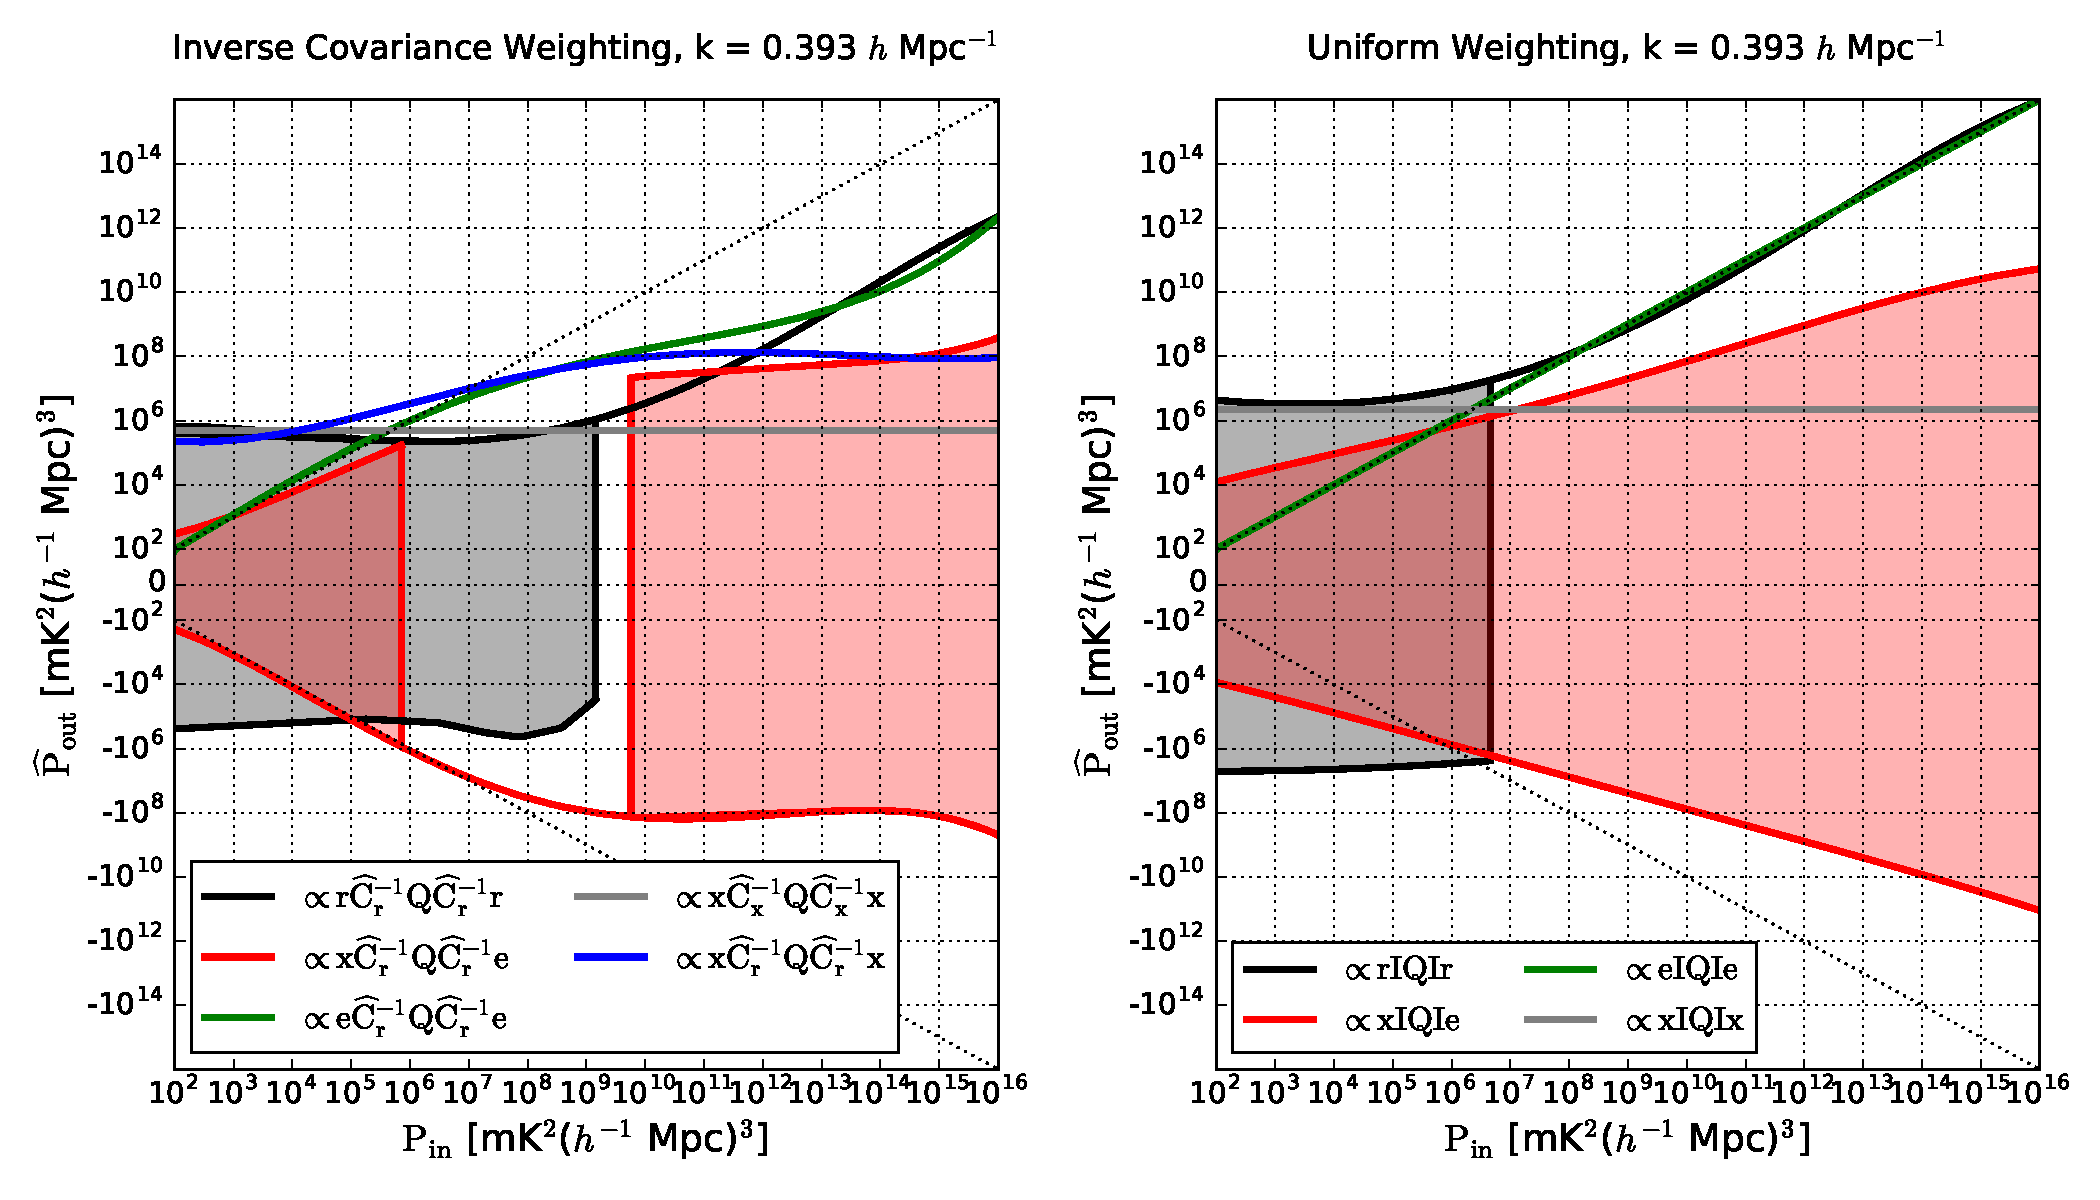
\includegraphics[width=1\textwidth]{plots/sigloss_terms.pdf}
	\caption{Illustration of the power spectrum amplitude of five different power spectrum terms, each a function of visibility data ($\textbf{x}$), simulated injected EoR signal ($\textbf{e}$), or both ($\textbf{r}$). This figure shows how these quantities behave as the power level of the injected EoR signal increases (along the x-axis).  The details of the simulation used to generate the figure is explained in Chapter \ref{sec:Practice}; here we sample a larger $P_{\rm in}$ range and fit smooth polynomials to our data points to make an illustrative example. We emphasize that the output power spectrum in black ($\widehat{P}_{\rm out}=\widehat{\textbf{P}}_r$) approximates the (lossy) power spectrum estimate that is output by our analysis pipeline prior to any signal loss adjustments. Roughly speaking, it can be compared to the input signal level ($P_{\rm in}$) to estimate the amount of signal loss. Left: Empirical inverse covariance weighting is used in power spectrum estimation, as done in \citet{ali_et_al2015}. The dotted diagonal black line indicates perfect 1:1 input-to-output mapping (no signal loss). The gray horizontal line is the power spectrum value of data alone, $\widehat{\textbf{P}}_{x}$ (it does not depend on injected power). The green signal-signal component is the term used in \citet{ali_et_al2015} to estimate signal loss. It is significantly higher than $\widehat{\textbf{P}}_{r}$ (black) when the cross-terms (red) are large and negative (black $=$ green $+$ red $+$ blue). In the regime where cross-correlations between signal and data are not dominant (small and large $P_{\rm in}$), the cross-terms have a noise-like term with width $\sqrt{\widehat{\textbf{P}}_e}\sqrt{\widehat{\textbf{P}}_x}$. However, at power levels comparable to the data (the middle region), the cross-terms can produce large, negative estimates due to couplings between $\textbf{x}$ and $\textbf{e}$ which affect $\widehat{\textbf{C}}_{r}$. This causes the difference between the green curve (which exhibits negligible loss at the data-only power spectrum value) and the black curve (which exhibits $\sim4$ orders of magnitude of loss). Right: The same power spectrum terms illustrated for the uniform weighted case.}
\label{fig:sigloss_terms}
\end{figure*}

The source of the strong negative cross-term is not immediately obvious, however it is an explainable effect. 
When $\textbf{R}_{r}$
is taken to be $\widehat{\textbf{C}}_{r}^{-1}$, the third term of Equation \eqref{eq:crossterm} is a cross-correlation between $\widehat{\textbf{C}}_{r}^{-1}\textbf{x}$ and
$\widehat{\textbf{C}}_{r}^{-1}\textbf{e}$. As shown in \citet{switzer_et_al2015}, this cross-correlation term is non-zero, and in fact negative in expectation. 
This negative cross-term power arises from a coupling between the inverse of 
$\widehat{\textbf{C}}_{r}$ and $\mathbf{x}$. 
Intuitively, we can see this by expanding the empirical covariance of $\textbf{r}=\textbf{x}+\textbf{e}$:

\begin{eqnarray}
\widehat{\textbf{C}}_{r} &=& \langle \textbf{rr}^{\dagger} \rangle_{t} \nonumber \\ 
&=& \langle \textbf{xx}^{\dagger} \rangle_{t} + \langle \textbf{xe}^{\dagger} \rangle_{t} + \langle \textbf{ex}^{\dagger} \rangle_{t} + \langle 
\textbf{ee}^{\dagger} \rangle_{t},
\end{eqnarray}

\noindent where we can neglect the first term because $\textbf{x}$ is small (i.e., the large negative cross-term power in the left panel of Figure \ref{fig:sigloss_terms} occurs when the injected amplitude surpasses the level of the data-only power spectrum).  Without loss of generality, we will assume
an eigenbasis of $\textbf{e}$, so that $\langle 
\textbf{ee}^{\dagger} \rangle_{t}$ is diagonal. The middle 
two terms, however, can have power in their off-diagonal terms due to the fact that, when averaging over a finite
ensemble, $\langle\textbf{xe}^\dagger\rangle_t$ is not zero.  As shown in Appendix C of \citet{parsons_et_al2014}%\footnote{This same appendix also gives a now-prescient warning about signal loss and the dangers of noise and sample variance in inverse covariance.}
, to leading order the inversion of a diagonal-dominant matrix like $\widehat{\textbf{C}}_{r}$ (from $\langle 
\textbf{ee}^{\dagger} \rangle_{t}$) with smaller
off-diagonal terms results in a new diagonal-dominant matrix with negative off-diagonal terms. These off-diagonal
terms depend on both $\textbf{x}$ and $\textbf{e}$. Then, when $\widehat{\textbf{C}}^{-1}_{r}$ is multiplied into $\textbf{x}$,
the result is a vector that is similar to $\textbf{x}$ but
contains a residual correlation to $\textbf{e}$ from the off-diagonal components of $\widehat{\textbf{C}}^{-1}_{r}$. The
correlation is negative because the product $\widehat{\textbf{C}}_r^{-1}\textbf{x}$ effectively squares the $\textbf{x}$-dependence
of the off-diagonal terms in $\widehat{\textbf{C}}^{-1}_{r}$ while retaining the negative sign that arose from the inversion
of a diagonal-dominant matrix.

{\bf In general:} Another way to phrase the shortcoming of the empirical inverse covariance estimator is that it is not properly normalized. Signal loss due to couplings between the data and its weightings arise because our unnormalized quadratic estimator from Equation \eqref{eq:qhat} ceases to be a quadratic quantity, and instead contains higher order powers of the data. However, the normalization matrix $\mathbf{M}$ is derived assuming that the unnormalized estimator is quadratic in the data. The power spectrum estimate will therefore be incorrectly normalized, which manifests as signal loss. We leave a full analytic solution for $\mathbf{M}$ for future work, since our simulations already capture the full phenomenology of signal loss and have the added benefit of being more easily generalizable in the face of non-Gaussian systematics.

\subsection{Signal Loss in Practice}
\label{sec:Practice}

We now shift our attention towards computing upper limits on the EoR signal for the fringe-rate filtered PAPER-64 dataset in a way that accounts for signal loss. While our methodology 
outlined below is independent of weighting scheme, here we demonstrate the computation using empirically estimated inverse covariance weighting 
($\textbf{R} \equiv \widehat{\textbf{C}}^{-1}$), the weighting scheme used in \citetalias{ali_et_al2015} which leads to substantial loss. 

One issue to address is how one incorporates the randomness of $\widehat{P}_{\rm out}$ into our signal loss corrections. A different realization of the mock EoR signal is injected with each bootstrap run, causing the output to vary in three ways ---  there is noise variation from the bootstraps, there is cosmic variation from generating multiple realizations of the mock EoR signal, and there is a variation caused by whether the injected signal looks more or less ``like'' the data (i.e., how much coupling there is, which affects how much loss results). 

For each injection level, the true $P_{\rm in}$ is simply the average of our bootstrapped estimates $\widehat{P}_{\rm in}$, since $\widehat{P}_{\rm in, \alpha}$ is by construction an unbiased estimator. Phrased in the context of Bayes' rule, we wish to find the posterior probability distribution $p(P_{\rm in} | 
\widehat{P}_{\rm out})$, which is the probability of $P_{\rm in}$ given the uncorrected/measured power spectrum estimate $\widehat{P}_{\rm out}$.  Bayes' rule relates the posterior, which we don't know, to the likelihood, which we can forward model. In other words,

\begin{equation}
\label{eq:Bayes}
p(P_{\rm in} | \widehat{P}_{\rm out}) \propto {\mathcal{L} (  \widehat{P}_{\rm out} | P_{\rm in})}\,p(P_{\rm in}) ,
\end{equation}

\noindent where $\mathcal{L} $ is the likelihood function defined 
as the distribution of data plus signal injection ($\widehat{P}_{\rm out}$) given the injection $P_{\rm in}$.  We construct this distribution  
by fixing $P_{\rm in}$ and simulating our analysis pipeline for many realizations of the injected EoR signal 
consistent with this power spectrum. The resulting distribution is normalized such that the sum over $\widehat{P}_{\rm out}$ is unity, and the 
whole process is then repeated for a different value of $P_{\rm in}$. 

The implementation details of the injection process require some more detailed explanation. In our code, we add a new realization of EoR to each independent bootstrap of data (see Chapter \ref{sec:Boot} for a description of PAPER's bootstrapping routine) with the goal of simultaneously capturing cosmic variance, noise variance, and signal loss. To limit computing time we perform $20$ realizations of each $P_{\rm in}$ level. We also run $50$ total EoR injection levels, yielding $P_{\rm in}$ values that range from $\sim$$10^{5}$\,mK$^{2}$ ($h^{-1}$ Mpc)$^{3}$ to $\sim$10$^{11}$\,mK$^{2}$ ($h^{-1}$ Mpc)$^{3}$, resulting in a total of $1000$ data points on our $P_{\rm in}$ vs. $\widehat{P}_{\rm out}$ grid. 

Going forward, we treat every $k$-value separately in order to determine an upper limit on the EoR signal per $k$. We bin our simulation outputs along the $P_{\rm in}$ axis (one bin per injection level) and, since they are well-approximated by a Gaussian distribution in our numerical results, we smooth the distribution of $\widehat{P}_{\rm out}$ values by fitting Gaussians for each bin based on its mean and variance (and normalize them). Stitching all of them together results in a 2-dimensional transfer function --- the likelihood function in Bayes' rule, namely $\mathcal{L} (  \widehat{P}_{\rm out} | P_{\rm in})$. We then have a choice for our prior, $p(P_{\rm in})$, and we choose to invoke a Jeffreys prior (\citealt{jaynes1968}) because it is a true uninformative prior for a parameter space using Bayesian probability. %For a derivation and more details about the Jeffreys prior used in our analysis, see Appendix \ref{sec:jeffreys}.

The Jeffreys prior is defined as:

\begin{equation}
\label{eq:jeffreys}
p(P_{\rm in}) \propto \sqrt {\Bigg\langle \Bigg(\frac{\partial \mathcal{L}}{\partial P_{\rm in}} \Bigg)^{2}\Bigg\rangle},
\end{equation}

\noindent where

\begin{equation}
\label{eq:logprob}
\mathcal{L} = \mathrm{ln} \, p(\widehat{P}_{\rm out} | P_{\rm in}),
\end{equation}

\noindent recalling that in our framework $P_{\rm in}$ is the power spectrum of the EoR signal (uniformly weighted), and $\widehat{P}_{\rm out}$ is the weighted output power spectrum of the data plus EoR.

Since, for a single injection amplitude, our bootstrapped $\widehat{P}_{\rm out}$ values are well-approximated by a Gaussian distribution, we can write: 

\begin{equation}
\label{eq:prob}
p(y | x) = \frac{1}{\sigma(x) \sqrt{2\pi}} e^{-\frac{1}{2}\big(\frac{y-\bar y(x)}{\sigma}\big)^{2}},
\end{equation}

\noindent simplifying our notation so that $x = P_{\rm in}$, $y = \widehat{P}_{\rm out}$, $\sigma$ is the standard deviation of $\widehat{P}_{\rm out}$, and $\bar y$ is the mean of $\widehat{P}_{\rm out}$. Using Equations \eqref{eq:prob} and \eqref{eq:logprob}, the quantity inside the expectation value of Equation \eqref{eq:jeffreys} becomes:

\begin{eqnarray}
\Big(\frac{\partial \mathcal{L}}{\partial x} \Big)^{2} &=& \frac{1}{\sigma^{2}}\Big(\frac{\partial \sigma}{\partial x}\Big)^{2} -  \Big(\frac{2(y-\bar y)}{\sigma^{3}}\Big)\frac{\partial \sigma}{\partial x}\frac{\partial \bar y}{\partial x} - \Big(\frac{2(y-\bar y)^{2}}{\sigma^{4}}\Big)\Big(\frac{\partial \sigma}{\partial x}\Big)^{2} \nonumber \\
&+& \Big(\frac{(y-\bar y)^{2}}{\sigma^{4}}\Big)\Big(\frac{\partial \bar y}{\partial x}\Big)^{2} + \Big(\frac{2(y-\bar y)^{3}}{\sigma^{5}}\Big)\frac{\partial \sigma}{\partial x}\frac{\partial \bar y}{\partial x} + \Big(\frac{(y-\bar y)^{4}}{\sigma^{6}}\Big)\Big(\frac{\partial \sigma}{\partial x}\Big)^{2}.
\end{eqnarray}

Taking the expectation value then removes all terms with odd powers of $(y - \bar y)$ because those Gaussian moments evaluate to zero. Additionally, the second moment can be simplified since $\langle (y - \bar y)^{2} \rangle = \sigma^{2}$ and the fourth moment can be simplified since $\langle (y - \bar y)^{4} \rangle = 3\sigma^{4}$. Finally, after some additional simplification the Jeffreys prior becomes:

\begin{equation}
\label{eq:jeffreys_final}
p(x) \propto \sqrt{ \frac{1}{\sigma^{2}}\Big(2\Big(\frac{\partial \sigma}{\partial x}\Big)^{2} + \Big(\frac{\partial \bar y}{\partial x}\Big)^{2}\Big) }.
\end{equation}

When we simulate our full injection framework, we note that the prior is set to zero outside our injection range. For the injections that we do sample, we can simply fit analytic functions to the mean and standard deviations of $\widehat{P}_{\rm out}$ ($\bar y$ and $\sigma$) as functions of $P_{\rm in}$. An example of the typical shape of these functions for the PAPER-64 analysis is shown in Figure \ref{fig:jeffreys1}, though in practice we fit solutions for every $k$-value and simulation independently.

\begin{figure}
	\centering
	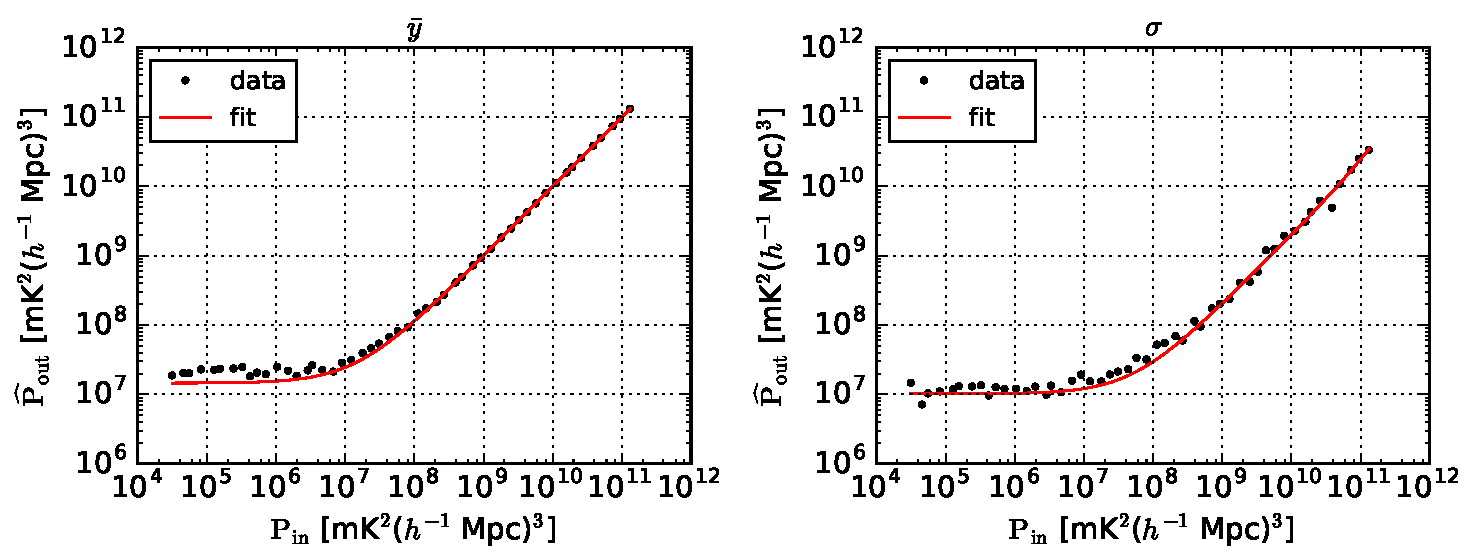
\includegraphics[width=\columnwidth]{plots/jeffrey_fits.pdf}
	\caption{An illustrative example (for the PAPER-64 analysis using uniform weighting and $k=0.393$\,$h$ Mpc$^{-1}$) of how the mean of $P_{\rm out}$ (left) and standard deviation of $P_{\rm out}$ (right) behave as a function of $P_{\rm in}$. Polynomials are fit to each (red) to describe how $\bar y$ and $\sigma$ evolve with $x$ (injection level), respectively, for the computation of the Jeffreys prior as defined in Equation \eqref{eq:jeffreys_final}. The polynomial fits for this example are $y = (-5.1 \times 10^{-15})x^{2} + x + (1.5 \times 10^{7})$ and $y = (5.0 \times 10^{-13})x^{2} + 0.2 x + 10^{7}$ for $\bar y$ and $\sigma$, respectively.}
	\label{fig:jeffreys1}
\end{figure}

We also show the typical shape of the Jeffreys prior used in our analysis in Figure \ref{fig:jeffreys2}, as computed by Equation \eqref{eq:jeffreys_final}. Most noticeably, it is not constant with $P_{\rm in}$, meaning a uniform prior, which is often used for simplicity, is informative in our application. Therefore, due to its objective nature we choose to use a Jeffreys prior in our analysis, multiplying our likelihood functions by Equation \eqref{eq:jeffreys_final} before computing posterior distributions.

\begin{figure}
	\centering
	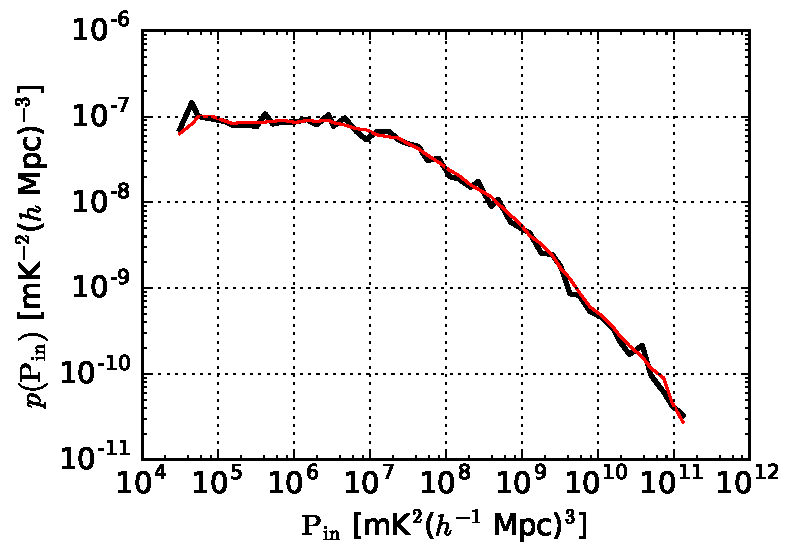
\includegraphics[width=10cm]{plots/jeffrey_prior.pdf}
	\caption{An example of the typical Jeffreys prior shape for the PAPER-64 analysis as computed by Equation \eqref{eq:jeffreys_final} (black). We smooth the prior using a sliding boxcar average over every $5$ injection levels (red). Most noticeably, the Jeffreys prior is not constant with $P_{\rm in}$, meaning a uniform prior would be an informative prior.}
	\label{fig:jeffreys2}
\end{figure}

Finally, our transfer functions are shown in Figure \ref{fig:sigloss_transfercurve} for both the weighted (left) and unweighted (right) cases. Our bootstrapped power spectrum outputs are shown as black points and the colored heat-map overlaid on top is the likelihood function modified by our prior. Although we only show figures for one $k$-value, we note that 
the shape of the transfer curve is similar for all $k$'s. We then invoke Bayes' interpretation and re-interpret it as the posterior $p(P_{\rm in}|\widehat{P}_{\rm out})$ where we recall that $\widehat{P}_{\rm out}$ represents a (lossy) power spectrum. To do this we make a horizontal cut across at the data value $\widehat{\textbf{P}}_{x}$ (setting $\widehat{P}_{\rm out} = \widehat{\textbf{P}}_{x}$), shown by the gray solid line, to yield a posterior distribution for the signal. We normalize this final distribution and compute the $95\%$ confidence interval (an upper limit on EoR).

By-eye inspection of the transfer function in Figure \ref{fig:sigloss_transfercurve} gives a sense of what the signal loss result should be. The power spectrum value of our data, $
\widehat{\textbf{P}}_{x}$ is marked by the solid gray horizontal lines. From the left plot (empirically estimated inverse covariance weighting), one can eyeball that a data value of $10^{5} \,$mK$^{2}$ ($h^{-1}$ Mpc)$^{3}$, for example, would map approximately to an upper limit of $\sim10^{9} \,$mK$^{2}$ ($h^{-1}$ Mpc)$^{3}$, implying a signal loss factor of $\sim10^{4}$. 

\begin{figure*}
	\centering
	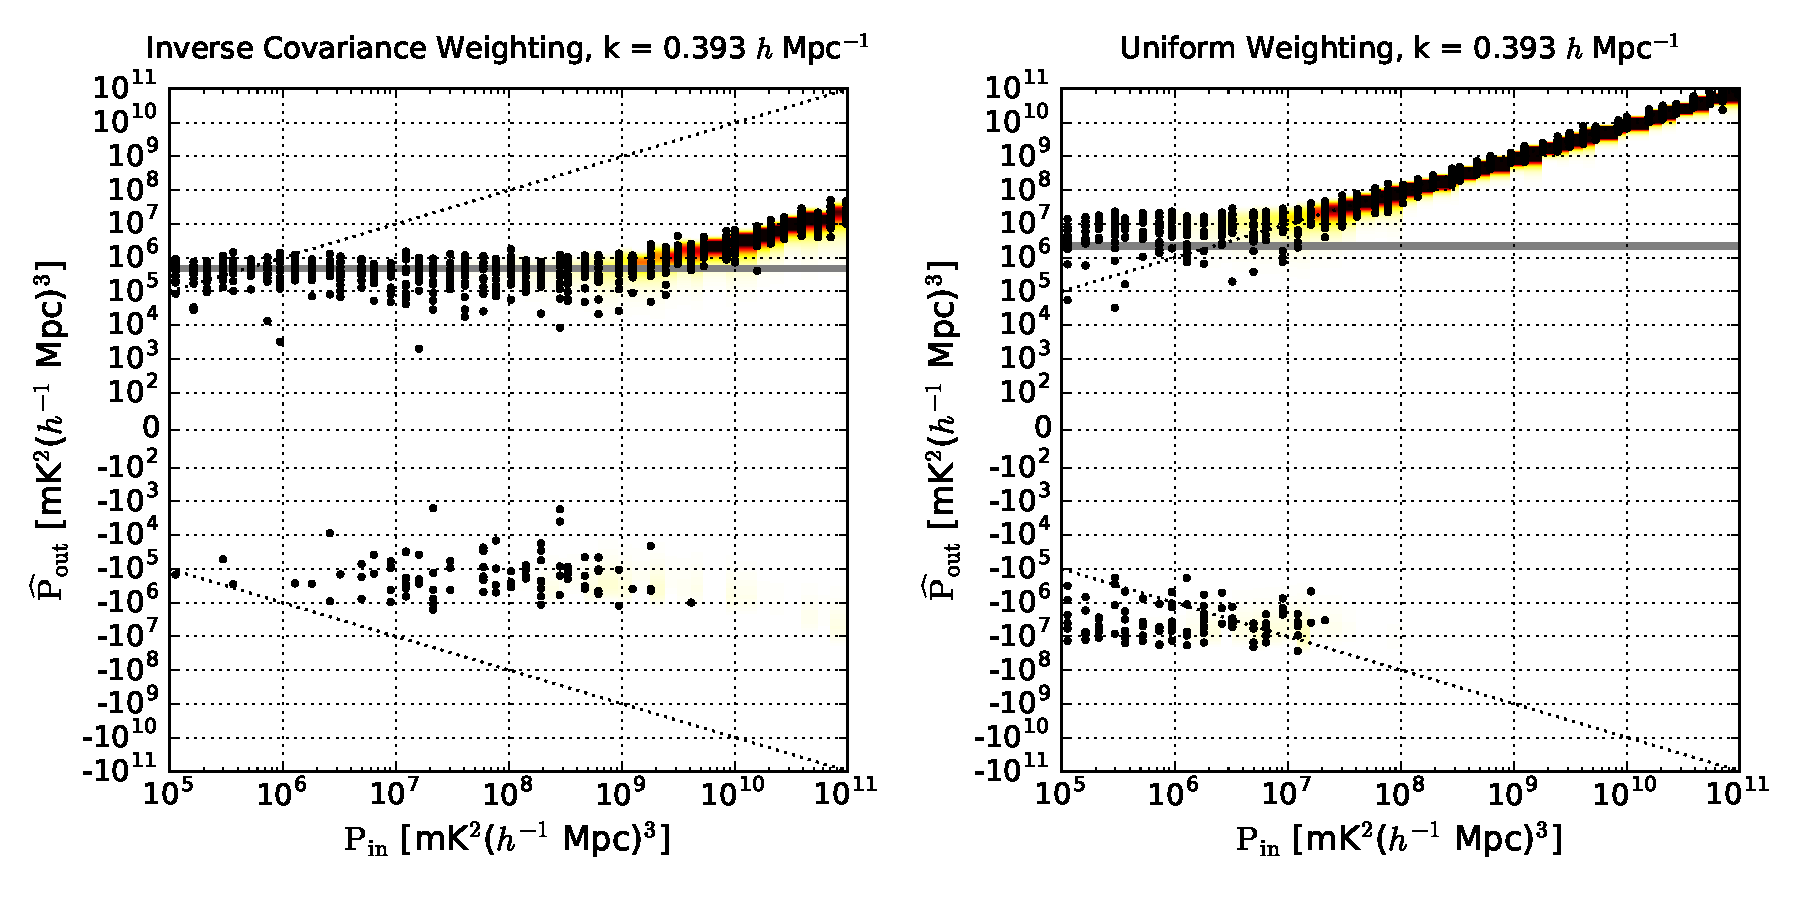
\includegraphics[width=1\textwidth]{plots/sigloss_transfercurve_posneg.pdf}
	\caption{Signal loss transfer functions showing the relationship of $P_{\rm in}$ and $\widehat{P}_{\rm out}$, as defined by Equations \eqref{eq:Pin} and \eqref{eq:sigloss}. Power spectra values (black points) are generated for $20$ realizations of $\textbf{e}$ per signal injection level. Since our $\widehat{P}_{\rm out}$ values are well-approximated by a Gaussian distribution, we fit Gaussians to each injection level based on the mean and variance of the simulation outputs. This entire likelihood function is then multiplied by a Jeffreys prior for $p(P_{\rm in}$), with the final result shown as the colored 
heat-maps on top of the points. Two cases are displayed: empirically estimated inverse covariance weighted PAPER-64 data (left) and uniform-weighted data (right). The dotted black 
diagonal lines mark a perfect unity mapping, and the solid gray horizontal line denotes the power spectrum value of the data $\widehat{\textbf{P}}_{x}$, from which a posterior distribution for the signal is extracted. From these plots, it is clear that the weighted case results in $\sim4$ orders of magnitude of signal loss at the data-only power spectrum value, whereas the uniform-weighted case does 
not exhibit loss. The general shape of these transfer functions are also shown by the black curves in Figure \ref{fig:sigloss_terms} for comparison.}
	\label{fig:sigloss_transfercurve}
\end{figure*}

The loss-corrected power spectrum limit for empirically estimated inverse covariance weighted PAPER-64 data is shown in Figure \ref{fig:ps2_data} (solid red), which we can compare to the original lossy result (dashed red). Post-signal loss estimation, the power spectrum limits are higher than both the theoretical noise level (green) and uniform-weighted power spectrum (which is shown three ways: black and gray points are positive and negative power spectrum values, respectively, with $2\sigma$ error bars from bootstrapping, the solid blue is the upper limit on the EoR signal using the full signal injection framework, and the shaded gray is the power spectrum values with thermal noise errors). We elaborate on this point in the next section, as well as investigate alternate 
weighting schemes to inverse covariance weighting, with the goal of finding one that balances the aggressiveness of down-weighting contaminants and minimizing the loss of the EoR signal. 

\begin{figure*}
	\centering
	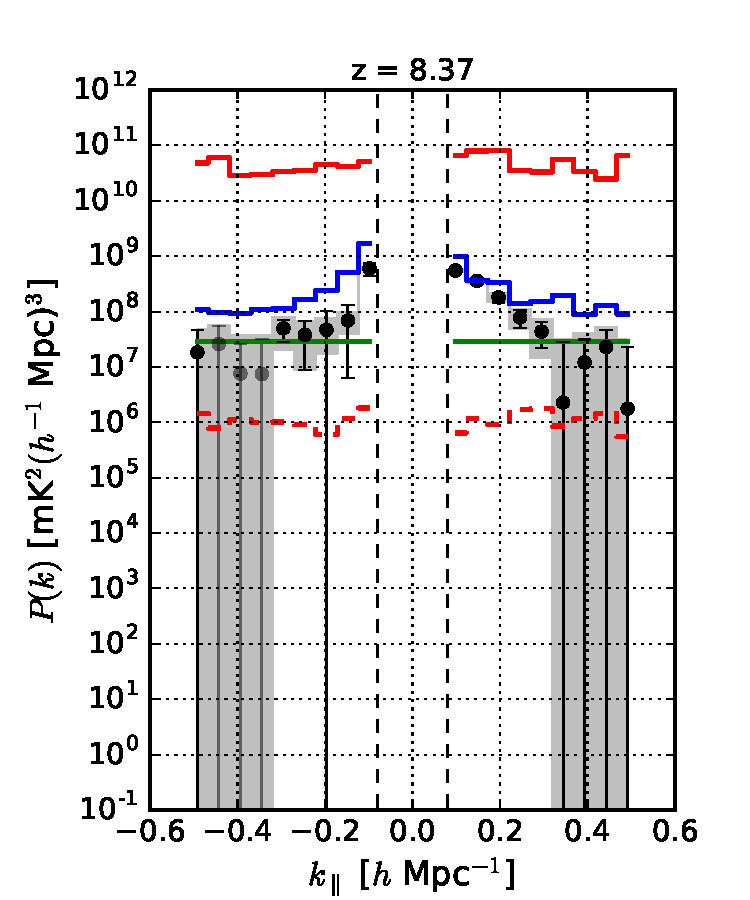
\includegraphics[width=0.45\textwidth]{plots/ps1_data.pdf}
	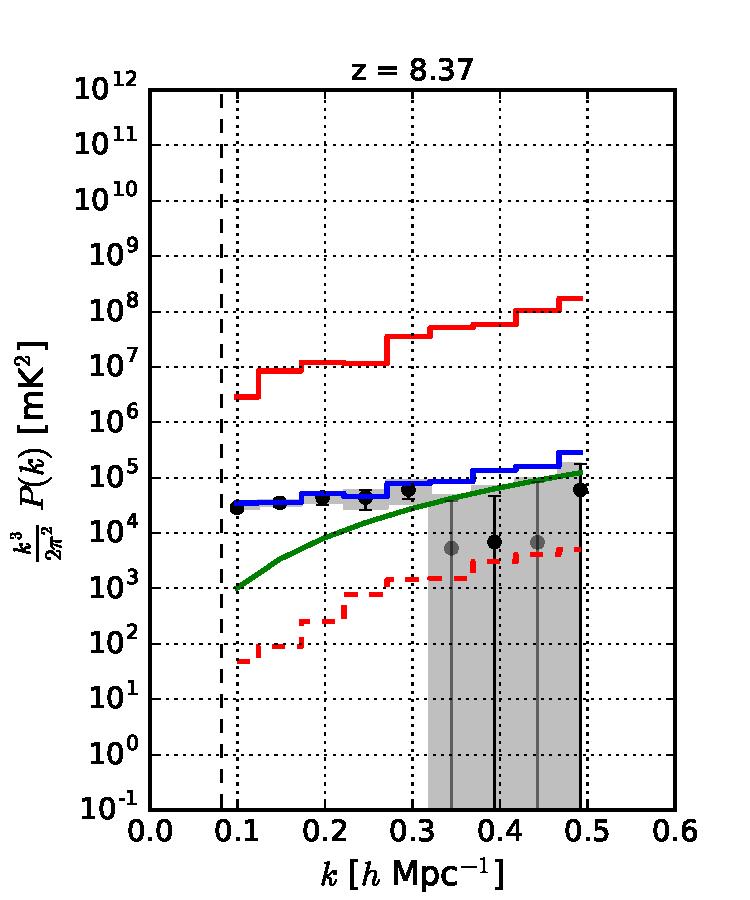
\includegraphics[width=0.45\textwidth]{plots/ps2_data.pdf}
	\caption{A power spectrum of a subset of PAPER-64 data illustrating the use of empirical inverse covariance weighting. The solid red curve is the $2\sigma$ upper limit on the EoR signal estimated from our signal injection framework using empirical inverse covariance weighting. Shown for comparison is the lossy limit prior to signal loss estimation (dashed red). The theoretical $2\sigma$ thermal noise level prediction based on observational parameters is in green, whose calculation is detailed in Chapter \ref{sec:Error}. Additionally, the power spectrum result for the uniform weighted case is shown in three different ways: power spectrum values (black and gray points as positive and negative values, respectively, with $2\sigma$ error bars from bootstrapping), the $2\sigma$ upper limit on the EoR signal using our full signal injection framework (solid blue), and the measured power spectrum values with $2\sigma$ thermal noise errors (gray shaded regions). The vertical dashed black lines signify the horizon limit for this analysis using $30$\,m baselines. In this example, we see that the lossy power spectrum limit is $\sim 4$ orders of magnitude too low when using empirical inverse covariance weighting.}
\label{fig:ps2_data}
\end{figure*}

\subsection{Minimizing Signal Loss}
\label{sec:Weight}

With a signal loss formalism established, we now have the capability of experimenting 
with different weighting options for $\textbf{R}$. Our goal here is to choose a weighting method that successfully down-weights 
foregrounds and systematics in our data without generating large amounts of signal loss as we have seen with the inverse covariance estimator. We have found that the balance 
between the two is a delicate one and requires a careful understanding and altering of empirical covariances. 

We saw in Chapter \ref{sec:otherweight} how limiting the number of down-weighted eigenmodes (i.e., flattening out part of the 
eigenspectrum and effectively decoupling the lowest-valued eigenmodes, which are typically EoR-dominated, from the data) can help minimize signal loss. We experiment with this idea on PAPER-64 data, dialing the number of modes 
that are down-weighted from zero (which is equivalent to identity-weighting, or the uniform-weighted case) to $21$ (which is the full inverse 
covariance estimator). The power spectrum results for one $k$-value, both before and after signal loss 
estimation, are shown in the top panel in Figure \ref{fig:sigloss_modeloop}. We see that the amount of signal loss increases as weighting 
becomes more aggressive (dashed red). In other words, more EoR-dominated fluctuations are being overfit and 
subtracted as more modes are down-weighted. We also find that the power spectrum upper limit, post-signal loss estimation, 
increases with the number of down-weighted modes (solid red). The more modes we use in down-weighting, the stronger the coupling between the weighting and the data, and the greater the error we have in estimating the power spectrum. \citet{switzer_et_al2013} took a similar approach in determining the optimal number of modes to down-weight in GBT data, finding similar trends and noting that removing too few modes is limited by residual foregrounds and removing too many modes is limited by large error bars and signal loss.

Optimistically, we expect there to be a ``sweet spot" as we dial our regularization knob; a level of regularization where weighting 
is beneficial compared to uniform weighting (blue). In other words, we would like a weighting scheme that down-weights eigenmodes that predominantly describe foreground modes, but not EoR modes. We see in Figure \ref{fig:sigloss_modeloop} that this occurs roughly when 
only the $\sim3$ highest-valued eigenmodes are down-weighted and the rest are given equal weights (though for the case shown, weighting only slightly outperforms uniform weighting). For a similar discussion on projecting out modes (zeroing out eigenmodes, rather than just ignoring their relative weightings as we do in this study), see \citet{switzer_et_al2013}. 

We also saw in Chapter \ref{sec:otherweight} how adding the identity matrix to the empirical covariance can minimize signal loss. We experiment with this idea as well, shown in the bottom panel of Figure \ref{fig:sigloss_modeloop}. The dashed red and solid red lines represent power spectrum limits pre and post-signal loss estimation, respectively, as a function of the strength of $\textbf{I}$ that is added to $\widehat{\textbf{C}}$, quantified as a percentage of Tr($\widehat{\textbf{C}})\textbf{I}$ added to $\widehat{\textbf{C}}$. We parameterize this ``regularization strength" parameter as $\gamma$, namely $\widehat{\textbf{C}} \equiv \widehat{\textbf{C}} + \gamma$Tr$(\widehat{\textbf{C}})\textbf{I}$. From this plot we see that only a small percentage of Tr($\widehat{\textbf{C}})$ is needed to significantly reduce loss. We expect that as the strength of $\textbf{I}$ is increased (going to the left), both the red curves will approach the uniform-weighted case. We also notice that the post-signal loss limit hovers around the uniform-weighted limit for a large range of regularization strengths and while an overall trend from high-to-low signal loss is seen as the strength increases, there does not appear to be a clear ``minimum" that produces the least loss.

\begin{figure*}
	\centering
	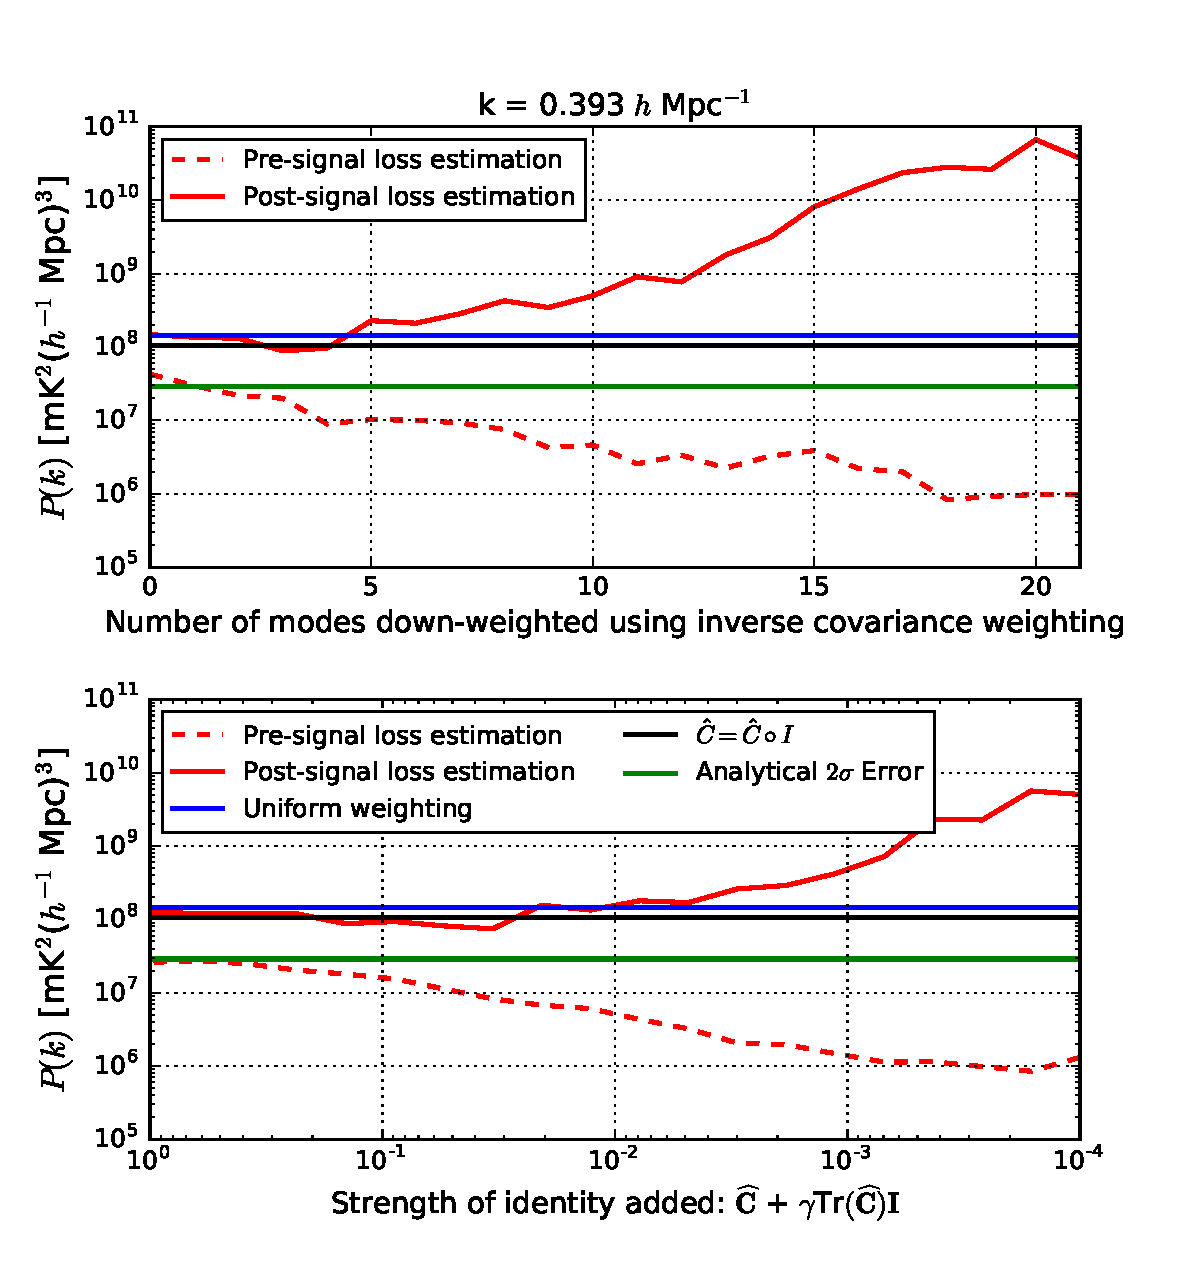
\includegraphics[width=.7\textwidth]{plots/sigloss_modeloop_2panel.pdf}
	\caption{Power spectra $2\sigma$ upper limits for $k=0.393$\,$h$ Mpc$^{-1}$ for fringe-rate filtered PAPER-64 data. Top: Values 
are shown before (dashed red) and after (solid red) signal loss estimation via our signal injection framework as a function of number of eigenmodes of $\widehat{\textbf{C}}$ that 
are down-weighted. This regularization knob is tuned from $0$ modes on the left (i.e., unweighted) to $21$ modes on the right (i.e., the full inverse 
covariance estimator). $\sim4$ orders of magnitude of signal loss results when using empirically estimated inverse covariance weighting. Bottom: Power spectrum upper limits before (dashed red) and after (solid red) signal loss estimation as a function of identity added to the empirical covariance. This regularization knob is tuned from $\gamma = 10^{-4}$ on the right (i.e., very little regularization) to $\gamma = 1$ on the left (see main text for the definition of $\gamma$). Also 
plotted in both panels for comparison are $2\sigma$ power spectrum upper limits for the uniform-weighted case (blue) and inverse variance 
weighted case (black); both are after signal loss estimation. Finally, a theoretical prediction for noise ($2\sigma$ error) is plotted 
as green. In the PAPER-64 analysis in this chapter, we choose to use a regularization scheme of $\widehat{\textbf{C}}_{\rm eff} \equiv 0.09 \, $Tr($\widehat{\textbf{C}})\textbf{I} + \widehat{\textbf{C}}$ ($\gamma = 0.09$) as a simple example of regularization that minimizes loss, and note that the power spectrum limits using this type of regularization are roughly constant across a large range of values of $\gamma$.}
	\label{fig:sigloss_modeloop}
\end{figure*}

In addition to our thermal noise prediction (green) and uniform-weighted power spectrum limit (blue), one additional horizontal line is shown in Figure \ref{fig:sigloss_modeloop} 
in both panels and represents a third regularization technique. This line (black) denotes the power spectrum value, post-signal loss estimation, for inverse variance weighting (multiplying an identity 
matrix element-wise to $\widehat{\textbf{C}}$). This result is single-valued and not a function of the horizontal axis. We see that all three regularization schemes shown (solid red top panel, solid red bottom panel, black) perform similarly at 
their best (i.e., when $\sim3$ eigenmodes are down-weighted in the case of the top panel's solid red curve). However, for the remainder of this chapter, we choose to use the weighting option of $\widehat{\textbf{C}} + 0.09 \,$Tr($\widehat{\textbf{C}})\textbf{I}$, or $\gamma = 0.09$, which we will denote as $\widehat{\textbf{C}}_{\rm eff}$. We choose this weighting scheme merely as a simple example of regularizing PAPER-64 covariances, noting that the power spectrum upper limit remains roughly constant for a broad range of values of $\gamma$. 

It is important to note that our signal injection methodology for assessing loss makes the assumption that we know the true signal's strength and structure. Realistically, these details about the EoR signal are unknown and our signal loss framework is limited by our simulations. Therefore, while this chapter employs this methodology as an example of one way of estimating loss, Chapter \ref{c.PSA64_results} uses uniform weightings in order to produce more trustworthy, straightforward power spectrum limits that do not suffer from loss.

The power spectrum result for our subset of PAPER-64 data (using only one baseline separation type, $10$ baselines, and $\widehat{\textbf{C}}_{\rm eff}$) using the analysis presented in this chapter is shown in Figure 
\ref{fig:ps1_data}. Again, the solid red curve represents our upper limit on the EoR signal using the full signal injection framework. The uniform weighted case is shown as the black and gray points, which correspond to positive and negative power spectrum values respectively (with 
$2\sigma$ errors bars from bootstrapping). It is also shown as an upper limit using the signal injection framework (solid blue), which is interestingly larger than the errors computed from bootstrapping, likely because the full injection framework takes into account additional sample variance whereas the bootstrapped errors do not. Finally, the gray shaded regions combine the measured uniform weighted power spectrum values with thermal noise errors. We show this power spectrum result as one example of how a simple regularization of an empirical covariance matrix can minimize signal loss, though we also note that this weighting does not produce more stringent limits than the uniform weighted case, thus further motivating uniform-weighting for our revised results in Chapter \ref{c.PSA64_results}. 

\begin{figure*}
	\centering
	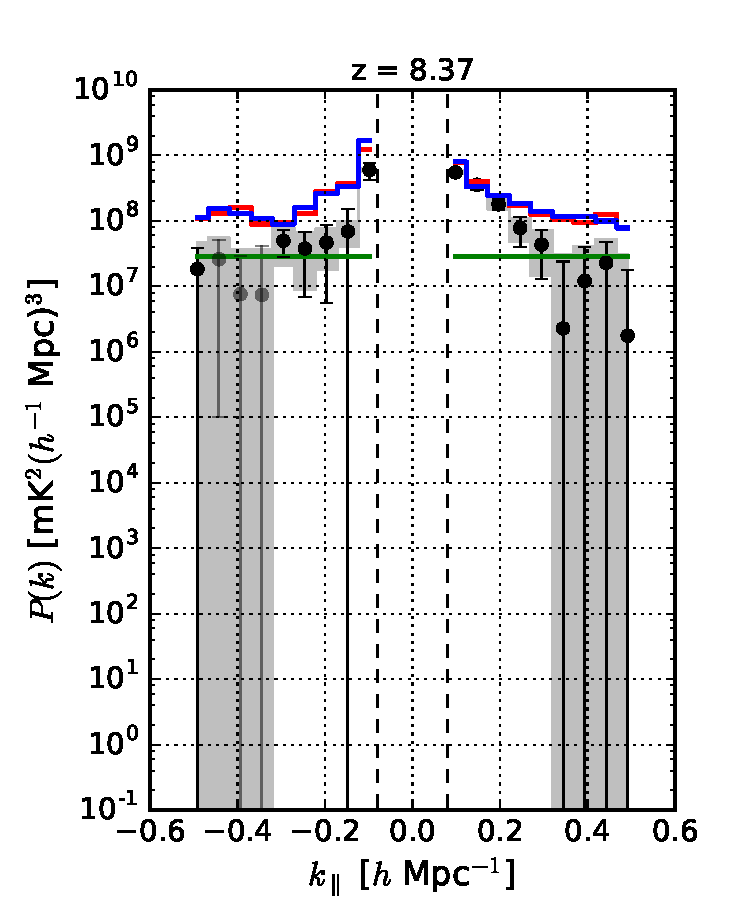
\includegraphics[width=0.45\textwidth]{plots/ps1_data_add.pdf}
	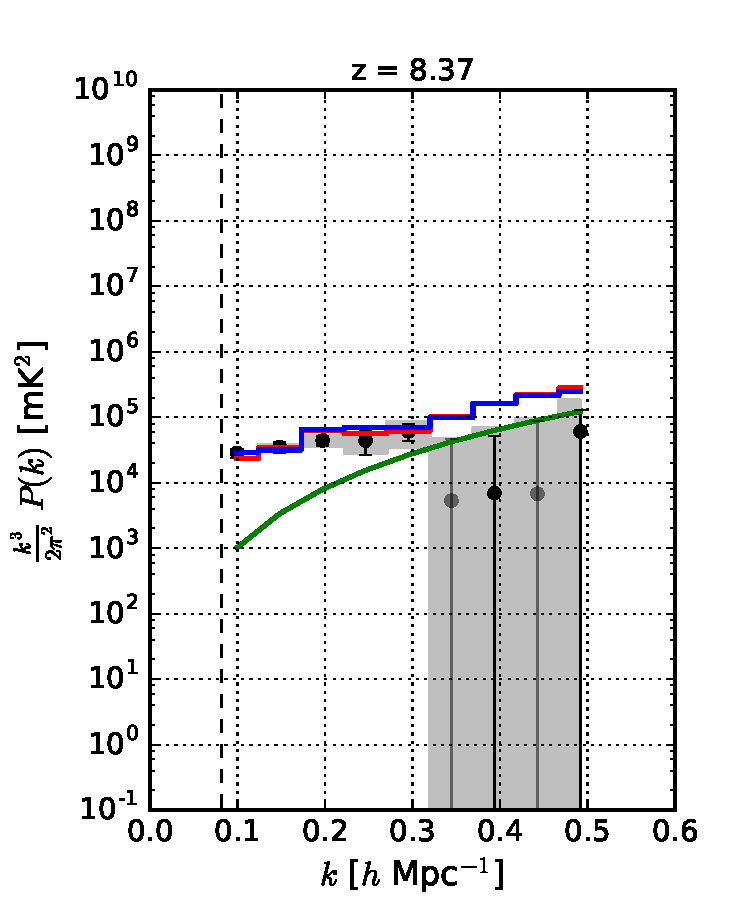
\includegraphics[width=0.45\textwidth]{plots/ps2_data_add.pdf}
	\caption{A power spectrum of a subset of PAPER-64 data illustrating the use of $\widehat{\textbf{C}}_{\rm eff}$ to minimize signal loss. The solid red curve is the $2\sigma$ upper limit on the EoR signal estimated from our signal injection framework. The theoretical $2\sigma$ thermal noise level prediction based on observational parameters is in green. Additionally, the power spectrum result for the uniform weighted case is shown in three different ways: power spectrum values (black and gray points as positive and negative values, respectively, with $2\sigma$ error bars from bootstrapping), the $2\sigma$ upper limit on the EoR signal using our full signal injection framework (solid blue), and the measured power spectrum values with $2\sigma$ thermal noise errors (gray shaded regions). The vertical dashed black lines signify the horizon limit for this analysis using $30$\,m baselines. This power spectrum result does not use the full dataset's sensitivity as in \citet{ali_et_al2015} and Chapter \ref{c.PSA64_results}, though we include all analysis changes which have mostly stemmed from revisions regarding signal 
loss, bootstrapping, and the theoretical error computation. We see that the regularization scheme used here produces limits similar to the unweighted limits.}
	\label{fig:ps1_data}
\end{figure*}

In this section we have shown three simple ways of regularizing $\widehat{\textbf{C}}$ to minimize signal loss using PAPER-64 
data. There are many other weighting schemes that we leave for consideration in future work. For example, one could estimate 
$\widehat{\textbf{C}}$ using information from different subsets of baselines. For redundant arrays this might mean calculating $
\widehat{\textbf{C}}$ from a different but similar baseline type, such as the $\sim30$\,m diagonal PAPER baselines (instead of the 
horizontal E/W ones). Alternatively, covariances could be estimated from all baselines except the two being cross-multiplied 
when forming a power spectrum estimate. This method was used in \citet{parsons_et_al2014} (a similar method was also used in \citet{dillon_et_al2015}) in order to avoid suppressing the 
21\,cm signal, and it is worth noting that the PAPER-32 results are likely less impacted from the issue of signal loss underestimation 
because of this very reason (however, they are affected by the error estimation issues described in Chapter \ref{sec:Error}, so 
we also regard those results as suspect and superseded by those in Chapter \ref{c.PSA64_results}).

Another possible way to regularize $\widehat{\textbf{C}}$ is to use information from different ranges of LST. For example, one could 
calculate $\widehat{\textbf{C}}$ with data from LSTs where foregrounds are stronger (earlier or later LSTs than the ``foreground-quiet" range typically used in forming power spectra) --- doing so may yield a better description of the foregrounds that we desire to 
down-weight, especially if residual foreground chromaticity is instrumental in origin and stable in time. Fundamentally, each of these examples are similar in that they rely on a computation of $\widehat{\textbf{C}}$ from 
data that is similar but not exactly the same as the data that is being down-weighted. Ideally this would be effective in down-weighting shared contaminants yet avoid signal loss from overfitting EoR modes in the power spectrum dataset itself. 

In Chapter \ref{sec:CaseStudy}, we have detailed several aspects of signal loss in PAPER-64: how the loss arises, how it can be estimated from an injection framework, and ways it can be minimized. We again emphasize that these lessons learned about signal loss are largely responsible for shaping our revised analysis of PAPER data. In the remainder of this chapter, we will transition to other aspects of our analysis that have been revised since \citetalias{ali_et_al2015}.

\section{Error Estimation}
\label{sec:Error}

Underestimated signal loss is the main reason for the revision of the power spectrum limits from \citetalias{ali_et_al2015}. It is interesting to note that --- had all the other aspects of the original analysis been correct --- the underestimated limits may have been more easily caught. Unfortunately, two related power spectrum components, namely the error bars on the power spectrum data points and the theoretical noise prediction, were also calculated incorrectly.

In this section, we summarize multiple inconsistencies and errors that have been found since the previous analysis in terms of error estimation. We first describe updated methods regarding bootstrapping, which determines the error bars on our limits. We then highlight an updated calculation for the theoretical noise sensitivity of PAPER-64 and illustrate how our revised calculation has been verified through simulations. 

\subsection{Bootstrapping}
\label{sec:Boot}

Broadly speaking, we desire robust methods for determining accurate 
confidence intervals for our measurements. For PAPER's analysis, we choose a data-driven method of error estimation, computing error bars that have been derived from the inherent 
variance of our measurements. A common technique used to do this is bootstrapping, which we first define below and then discuss its application to PAPER.

Bootstrapping uses sampling with replacement to estimate a posterior distribution. For example, bootstrap measurements (of power spectra, for example) can be made from different random samples of data. Each of these bootstraps is a different realization drawn from some underlying distribution, and realizations are correlated with each other to a degree set by the fraction of sampled points that are held in common between them. Through the process of re-sampling and averaging along different axes of a dataset, such as along baselines or times, we can estimate error bars for our results which represent the underlying distribution of values that are allowed by our measurements (\citealt{efron_tibshirani1994}; \citealt{andrae2010}).

One major caveat of bootstrapping arises when working with correlated data. If, for example, a dataset has many repeated 
values inside it, this would be reflected in each bootstrap. The same value would be present multiple times within a bootstrap 
and also be present between bootstraps, purely because it has a more likely chance of being drawn if there are repeats of 
itself. Therefore, bootstrapping correlated data results in a smaller variation between bootstraps, and hence, underestimates 
errors. 

This is the precisely how errors were underestimated in PAPER-64. Because of fringe-rate filtering, which averages data in time to increase sensitivity, PAPER-64 data is correlated along the time axis. Hence, there are fewer independent samples after filtering, thus decreasing the variance of the bootstraps.

More specifically, the PAPER-64 pipeline outputs $20$ bootstraps (over baselines), each a $2$-dimensional power 
spectrum that is a function of $k$ and time. In \citetalias{ali_et_al2015}, a second round of bootstrapping occurred over the time axis, and a total of $400$ bootstraps were created in this step, each comprised of randomly selected values sampled with replacement (i.e., each of these bootstraps contained the same number of values as the number of time integrations, which, at $\sim$
$700$, greatly exceeds the approximate number of independent samples after fringe-rate filtering).
Means were then taken of the values in each bootstrap. Finally, power 
spectrum limits were computed by taking the mean and standard deviation over all the bootstraps. We emphasize again that in 
this previous analysis, the number of elements sampled per bootstrap greatly 
exceeded the number of independent LST samples, underestimating errors. A random draw of $700$ 
measurements from this dataset has many repeated values, and the variance between hundreds of these random 
samples is smaller than the true underlying variance of the data. 

Given our new understanding of the sensitivity of bootstraps to the number of elements sampled, we have removed the second 
bootstrapping step along time entirely and now simply bootstrap over the baseline axis. Power spectrum $2\sigma$ errors (computed from bootstrap variances) with and without this bootstrapping change for a fringe-rate filtered noise simulation are shown in Figure 
\ref{fig:data_errors} in black and gray, respectively. The estimates are uniformly weighted in order to disentangle the effects of bootstrapping from signal loss. As 
shown in the figure, when more elements are drawn for each bootstrap than the number of 
independent samples (by over-sampling elements along the time axis), repeated values begin to crop up and the apparent variation between bootstraps drops, resulting in limits (gray) below the predicted noise level (green). Using the revised bootstrapping method, where bootstrapping only occurs over the baseline axis, the limits (black) are shown to agree with the analytic prediction for noise. While Figure \ref{fig:data_errors} implies that errors, computed prior to our bootstrapping change (gray), are underestimated by a factor of $\sim$ $5$ in mK$^{2}$ for the noise simulation (whose creation details are outlined in the next section), in practice this factor is lower for the case of real data (a factor of $\sim$ $3$ in mK$^{2}$ instead), possibly due to the data being less correlated in time than the fringe-rate filtered noise in the simulation. 

In addition to learning how sample independence affects bootstrapped errors, we have made three additional changes to our bootstrapping procedure since \citetalias{ali_et_al2015}, summarized here:

\begin{itemize}

\item{A second change to our bootstrapping procedure is that we now bootstrap over baseline cross-products, instead of the baselines themselves. In the previous analysis, baselines were bootstrapped prior to forming cross power spectra, and using this particular ordering of operations (bootstrapping, then cross-multiplication) yields variances that have been found to disagree with predicted errors from bootstrapping using simulations. On the contrary, bootstrapping over cross power spectra ensures that we are estimating the variance of our quantity of interest (i.e., the power spectrum). This change, while fundamental in retaining the integrity of the bootstrapping method in general, alters the resulting power spectrum errors by factors of $<2$ in practice.}

\item{In \citetalias{ali_et_al2015}, individual baselines were divided into five independent groups, where no baselines were repeated in each group. Then, baselines within each group were averaged together, and the groups were cross-multiplied to form power spectra. This grouping method was used to reduce computational time, however upon closer examination it has been found that the initial grouping introduces an element of randomness into the final measurements --- more specifically, the power spectrum value fluctuates depending on how baselines are assigned into their initial groups. Our new approach removes this element of randomness at the cost of computational expense, as we now perform all baseline cross-products.}

\item{Finally, the last change from the \citetalias{ali_et_al2015} method is that our power spectrum points (previously computed as the mean of all bootstraps), are now computed as the power spectrum estimate resulting from not bootstrapping at all. More specifically, we compute one estimate without sampling, and this estimate is propagated through our signal loss computation (this estimate is $\widehat{\textbf{P}}_{x}$). The difference between taking the mean of the bootstrapped values and using the estimate from the no-bootstrapping case is small, but doing the latter ensures that we are forming results that reflect the estimate preferred by all our data.}

\end{itemize}

In summary, we have learned several lessons regarding bootstrapping and have revised our analysis procedure in order to determine error bars that correctly reflect the variance in our power spectrum estimates. Bootstrapping can be an effective and straightforward way to estimate errors of a dataset, however, bootstrapping as a means of estimating power spectrum errors from real fringe-rate filtered data requires knowledge of the number of independent samples, which is not always a trivial task. We have thus avoided this issue by removing one of our bootstrap axes, as well as updated several other details of our procedure to ensure accurate re-sampling and error estimation.

\begin{figure}
	\centering
	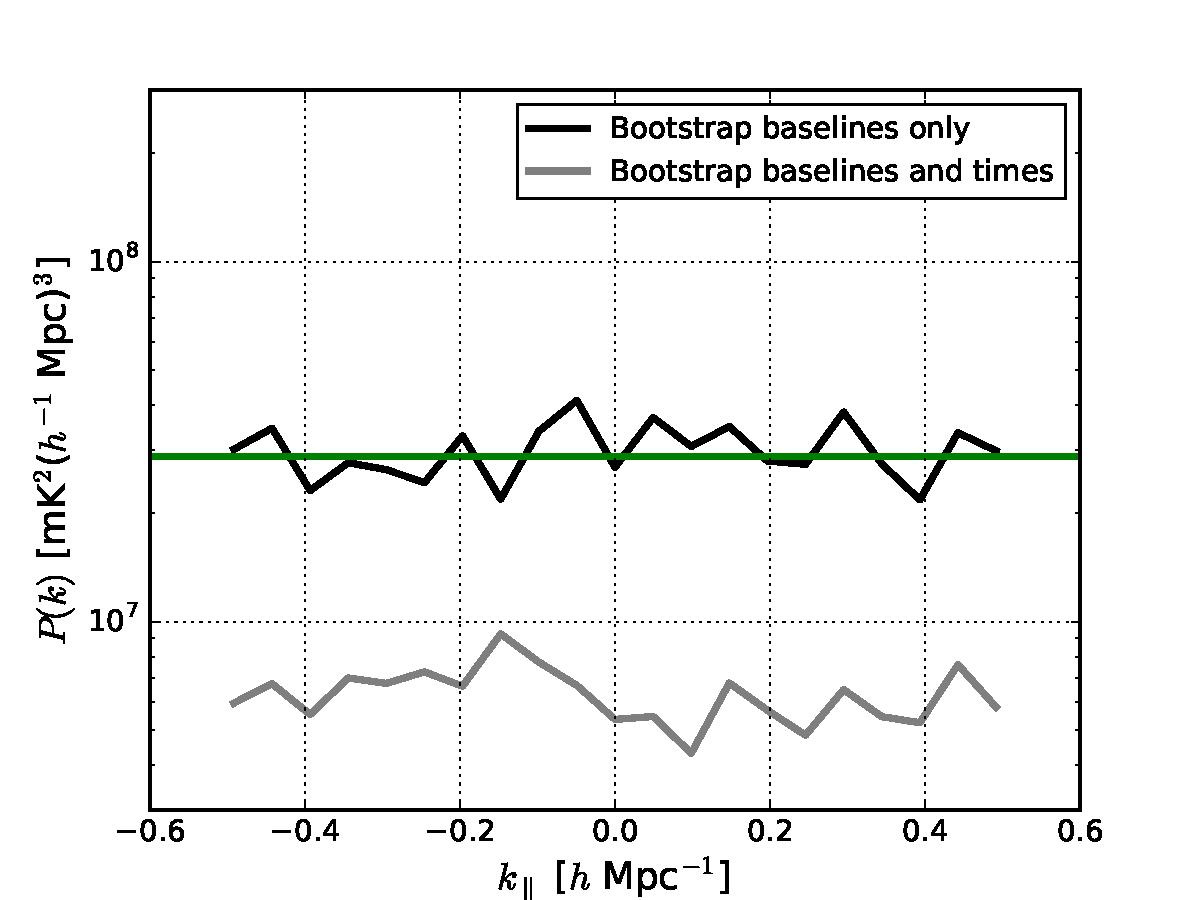
\includegraphics[trim={0.3cm 0cm 0.3cm 0.3cm},width=0.8\textwidth]{plots/noise_errors.pdf}
	\caption{$2\sigma$ power spectrum errors (from bootstrap variances) for a noise simulation (computed via Equation \eqref{eq:noise} using PAPER-64 observing parameters) using two different bootstrapping 
methods. The noise is fringe-rate filtered and a weighting matrix of $\textbf{I}$ (uniform-weighted) is used in order to disentangle the 
effects of bootstrapping from signal loss. The bootstrapping method used in \citet{ali_et_al2015} is shown in gray, where bootstrapping occurs along both the baseline and time axes. This underestimates errors by sampling more values than independent ones in the dataset (fringe-rate filtering reduces the number of independent samples along time). We use the method illustrated by the black curve in our updated analysis, where bootstrapping only occurs along the baseline axis. We find that these revised limits agree with the $2\sigma$ analytic prediction for noise (green).}
	\label{fig:data_errors}
\end{figure}

\subsection{Theoretical Error Estimation}
\label{sec:Error}

One useful way of cross-checking measured power spectrum values and errors is to compute a theoretical estimation of thermal noise based on observational parameters. Although a theoretical model often differs from true errors, it is helpful to understand the ideal case and the factors that affect its sensitivity. Upon re-analysis of PAPER-64, we have discovered that this estimate was also underestimated in previous analyses. 

To compute our theoretical noise estimate, we use an analytic sensitivity calculation. Through detailed studies using several independently generated noise simulations, what we found was that our simulations all agreed but were discrepant with the previous calculations. The analytic 
calculation is only an approximation and attempts to combine a large number of pieces of information in an approximate way; however, when re-considering some of the approximations, the differences were large enough (factors of $10$ in some cases) to warrant a 
careful investigation. What follows here is an 
accounting of the differences which have been discovered. We note that our theoretical error estimate, which is plotted as the solid green curve in many of the previous power spectrum plots in this thesis, is computed with these changes accounted for.

The noise prediction $n(k)$ (\citealt{parsons_et_al2012a}; \citealt{pober_et_al2013}) for a power spectral analysis of 
interferometric 21\,cm data, in temperature-units, is:

\begin{equation}
\label{eq:sense}
N(k) = \frac{X^{2}Y \Omega_{\rm eff} T_{\rm sys}^{2}}{\sqrt{2N_{\rm lst}N_{\rm seps}}\,t_{\rm int}N_{\rm days}N_{\rm bls}N_{\rm pols}}.
\end{equation}
We will now explain each factor in Equation \eqref{eq:sense} and highlight key differences from the numbers used in \citetalias{ali_et_al2015}.

\begin{itemize}
\item $X^{2}Y$: Conversion factors from observing coordinates (angles on the sky and frequency) to cosmological coordinates (co-moving 
distances). For $z=8.4$, $X^{2}Y = 5 \times 10^{11} \, h^{-3}$ Mpc$^{3}$ str$^{-1}$ GHz$^{-1}$.
\item $\Omega_{\rm eff}$: The effective primary beam area in steradians (\citealt{parsons_et_al2010}; \citealt{pober_et_al2012}). 
The effective beam area changes with the application of a fringe-rate filter, since different parts of the beam are up-weighted and down-weighted. Using numbers from Table 1 in \citet{parsons_et_al2016}, $\Omega_{\rm eff} = 0.74^{2}/0.24$ for an optimal fringe-rate 
filter and the PAPER primary beam. 
\item $T_{\rm sys}$: The system temperature is set by:

\begin{equation}
\label{eq:sys}
T_{\rm sys} = 180\Big(\frac{\nu}{0.18}\Big)^{-2.55} + T_{\rm rcvr},
\end{equation}

where $\nu$ are frequencies in GHz (\citealt{thompson_et_al2001}). We use a receiver temperature of $144$\,K, yielding $T_{\rm sys} = 431$\,K at $150$\,MHz. 
This is lower than the $T_{\rm sys}$ of $500$\,K used in \citetalias{ali_et_al2015} because of several small miscalculation errors that were 
identified\footnote{For example, there was a missing a square root in going from a variance to a standard deviation.}.
\item $\sqrt{2}$: This factor in the denominator of the sensitivity equation comes from taking the real part of the power spectrum 
estimates after cross-multiplying two independent visibility measurements. In \citetalias{ali_et_al2015}, a factor of $2$ was mistakenly used.
\item $N_{\rm lst}$: The number of independent LST bins that go into a power spectrum estimation. The sensitivity scales as the square root 
because we integrate incoherently over time. For PAPER-64, $N_{\rm lst} = 8$.
\item $N_{\rm seps}$: The number of baseline separation types (where baselines of a unique separation type have the same orientation and length) averaged incoherently in a final power spectrum estimate. For the 
analysis in this chapter, we only use one type of baseline (PAPER's 30\,m East/West baselines). However, both the updated limits in Chapter \ref{c.PSA64_results} and the sensitivity prediction in Figure \ref{fig:sense_check} use three separation types ($N_{\rm seps}=3$) to match \citetalias{ali_et_al2015}.
\item $t_{\rm int}$: Length of an independent integration of the data. It is crucial to adapt this number if filtering is applied along the time axis (i.e., a 
fringe-rate filter). We compute the effective integration time of our fringe-rate filtered data by scaling the original integration time $t_{i}$
using the following:
\begin{equation}
t_{\rm int} = t_{i} \frac{\int1 \, df}{\int w^{2}(f) \,df},
\end{equation}
where $t_{i}=43$ seconds, $t_{\rm int}$ is the fringe-rate filtered integration time, $w$ is the fringe-rate profile, and the integral is 
taken over all fringe-rates. For PAPER-64, this number is $t_{\rm int} = 3857$\,s. 
\item $N_{\rm days}$: The total number of days of data analyzed. In \citetalias{ali_et_al2015}, this number was set to $135$. However, because we 
divide our data in half (to form ``even" and ``odd" datasets, or $N_{\rm datasets} = 2$), this number should reflect the number of days in each individual dataset instead of the total. Additionally, this number should be adjusted to reflect the actual number of cross-multiplications that occur between datasets (``even" with ``odd" and ``odd" with ``even", but not ``odd" with ``odd" or ``even" with ``even" in order to avoid noise biases). Finally, because our LST coverage is not $100\%$ complete (it doesn't overlap for every single day), we incorporate a root-mean-square statistic in computing a realistic value of 
$N_{\rm days}$. Our expression therefore becomes:
\begin{equation}
N_{\rm days} = \sqrt{\langle N_{i}^{2}\rangle} \sqrt{(N_{\rm datasets}^{2}-N_{\rm datasets})}
 %\frac{1}{N_{\rm days}} = \sqrt{\Big\langle\frac{1}{N_{i}^{2}} \Big\rangle_{i}},
 \end{equation}
\noindent where $i$ indexes LST and frequency channel over all datasets (\citealt{jacobs_et_al2015}). For PAPER-64, our revised estimate of $N_{\rm days}$ is $\sim47$ 
days.
\item $N_{\rm bls}$: The number of baselines contributing to the sensitivity of a power spectrum estimate. In \citetalias{ali_et_al2015}, this number was 
the total number of $30$\,m East/West baselines used in the analysis. However, using the total number of baselines ($N_{\rm bls\_total} = 51$) neglects 
the fact that the \citetalias{ali_et_al2015} analysis averages baselines into groups for computational speed-up when cross-multiplying data. Our revised estimate for the parameter is:
\begin{equation}
N_{\rm bls} = \frac{N_{\rm bls\_total}}{N_{\rm gps}}\sqrt{\frac{N_{\rm gps}^{2}-N_{\rm gps}}{2}},
\end{equation}
\noindent where, in the \citetalias{ali_et_al2015} analysis, $N_{\rm gps} = 5$. Each baseline group averages down linearly as the number of baselines 
entering the group ($N_{\rm bls\_total}/N_{\rm gps}$) and then as the square root of the number of cross-multiplied pairs \Big($\sqrt{\frac{N_{\rm gps}^{2} - 
N_{\rm gps}}{2}}$\Big). A revised \citetalias{ali_et_al2015} analysis should therefore use $N_{\rm bls} \sim 32$ instead of $51$, and this change is taken into account in Figure \ref{fig:sense_check}. However, the analysis throughout this thesis no longer averages baselines into groups ($N_{\rm gps} = 1$). For the subset of data presented in this chapter, $N_{\rm bls} = 10$.
\item $N_{\rm pols}$: The number of polarizations averaged together. For the case of Stokes I, $N_{\rm pols}=2$.
\end{itemize}

An additional factor of $\sqrt{2}$ is gained in sensitivity when folding together positive and negative $k$'s to form $\Delta^{2}(k)$.

Our revised sensitivity estimate for the \citetalias{ali_et_al2015} analysis of PAPER-64 is shown in Figure \ref{fig:sense_check}. 
Together, the revised parameters yield a decrease in sensitivity (higher noise floor) by a factor of $\sim7$ in mK$^{2}$. 

\begin{figure}
	\centering
	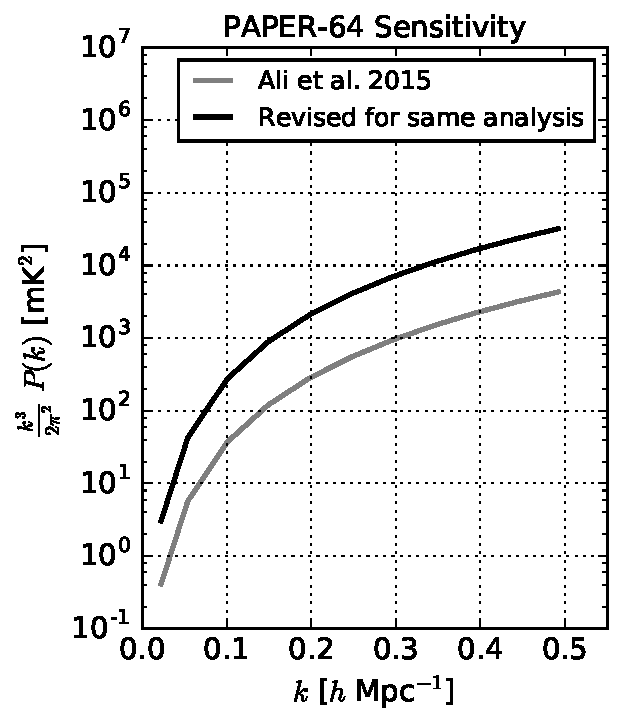
\includegraphics[width=0.55\textwidth]{plots/sense_check.pdf}
	\caption{An updated prediction for the thermal noise level of PAPER-64 data (black) is shown in comparison to previously 
published sensitivity limits (gray), both computed for the parameters and methods used in \citet{ali_et_al2015}. Major factors that contribute to the discrepancy are $
\Omega_{\rm eff}$, $N_{\rm days}$ and $N_{\rm bls}$, as in Equation \eqref{eq:sense} and described in Chapter \ref{sec:Error}, which when combined decreases our 
sensitivity (higher noise floor) by a factor of $\sim7$ in mK$^{2}$.}
	\label{fig:sense_check}
\end{figure}

To verify our thermal noise prediction, we form power spectra estimates using a pure noise simulation. We create Gaussian 
random noise assuming a constant $T_{\rm rcvr}$ (translated into $T_{\rm sys}$ via Equation \eqref{eq:sys}) but accounting for the true $N_{\rm days}$ as determined 
by LST sampling counts for each time and frequency in the LST-binned data. We convert $T_{\rm sys}$ into a root-mean-square variance statistic 
using:

\begin{equation}
\label{eq:noise}
T_{\rm rms} = \frac{T_{\rm sys}}{\sqrt{\Delta\nu \Delta t N_{\rm days} N_{\rm pols}}},
\end{equation}

\noindent where $\Delta\nu$ is the channel spacing, $\Delta t$ is the integration time, $N_{\rm days}$ is the number of daily counts for a 
particular time and frequency that went into our LST-binned set, and $N_{\rm pols}$ is the number of polarizations ($2$ for Stokes 
I). This temperature sets the variance of the Gaussian random noise.

Power spectrum results for the noise simulation, which uses our full power spectrum pipeline, are shown in Figure 
\ref{fig:ps_noise}. We highlight that the bootstrapped data (black and gray points, with $2\sigma$ error bars) and thermal noise prediction (solid green) show good agreement, as bootstrapping provides an accurate estimate of the noise variance. However, the limits from the full signal loss framework (weighted and unweighted in red and blue, respectively) are inflated, likely due to the additional inclusion of sample variance that comes from the EoR simulations. While the noise simulation provides an important indicator about the accuracy of our theoretical noise calculation, we note that the calculation did not take into account additional sources of error associated with earlier analysis steps (for example, \citet{trott_wayth_2017} show how calibration specifically can add errors to visibilities). Additionally, we recommend that future work investigate possible error correlations between baseline pairs and any interaction effects between signal and noise that may effect error calculations. Because of these reasons, we therefore interpret our noise prediction as the sensitivity floor for our measurements.

\begin{figure*}
	\centering
	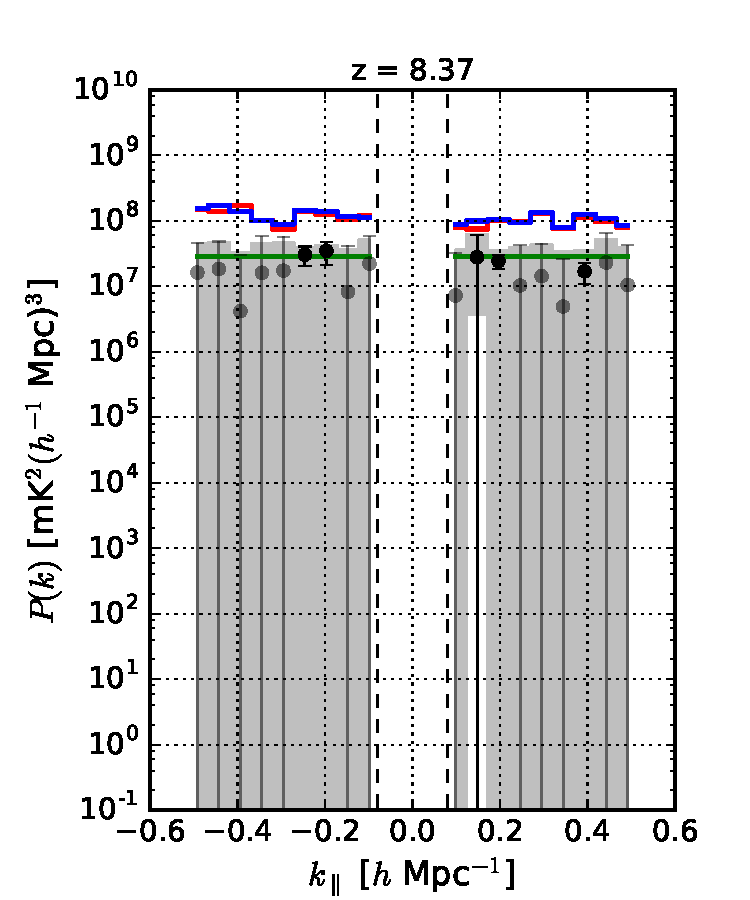
\includegraphics[width=0.45\textwidth]{plots/ps1_noise_add.pdf}
	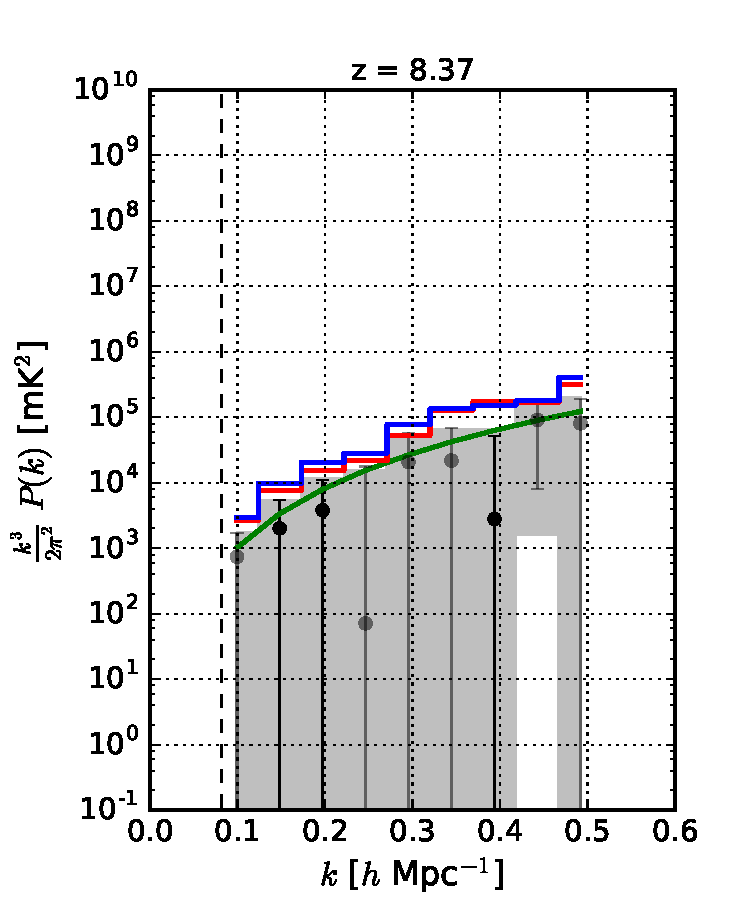
\includegraphics[width=0.45\textwidth]{plots/ps2_noise_add.pdf}
	\caption{The power spectrum for a noise simulation that mimics the noise level of a subset of PAPER-64 data, where the solid red curve is the $2\sigma$ upper limit on the EoR signal estimated from our signal injection framework using $\widehat{\textbf{C}}_{\rm eff}$. The theoretical $2\sigma$ thermal noise level prediction based on observational parameters (calculated by Equation \eqref{eq:sense}) is in green. Additionally, the power spectrum result for the uniform weighted case is shown in three different ways: power spectrum values (black and gray points as positive and negative values, respectively, with $2\sigma$ error bars from bootstrapping), the $2\sigma$ upper limit on the EoR signal using our full signal injection framework (solid blue), and the measured power spectrum values with $2\sigma$ thermal noise errors (gray shaded regions). The vertical dashed black lines signify the horizon limit for this analysis using $30$\,m baselines. We highlight that the bootstrapped data points and thermal noise prediction show good agreement, while the limits from the full injection framework (red and blue) are inflated due to the additional inclusion of sample variance that comes from the injection simulations.}
	\label{fig:ps_noise}
\end{figure*}

\section{Bias}
\label{sec:Bias}

In Chapter \ref{sec:BiasOverview} we highlighted some common sources of bias that can show up as power spectrum 
detections and imitate an EoR signal. We discussed the importance of using jackknife and null tests for instilling confidence in an EoR 
detection, as well as for identifying other sources of biases. Here we demonstrate methods used by PAPER-64 to mitigate 
foreground and noise bias and we perform null tests in order to characterize the stability and implications of our results.

\subsection{Mitigating Bias}
\label{sec:MitBias}

We briefly discuss one way we mitigate foreground leakage in a power spectrum estimate, and two ways we 
suppress noise biases. These methods are not novel to this analysis but here we frame them in the context of minimizing false 
(non-EoR) detections. 

Tailoring window functions is one way to suppress foreground biases (similar discussions to the following one are in \citet{liu_et_al2014b} and \citetalias{ali_et_al2015}). As alluded to in Chapter \ref{sec:SiglossOverview}, we 
have a choice for the normalization matrix $\textbf{M}$ in Equation \eqref{eq:phat}. For the analysis of PAPER-64 data, we 
compute $\textbf{M}$ using the matrix $\textbf{G}$ (which would be the Fisher matrix if $\textbf{R} \equiv \textbf{C}^{-1}$), defined as:

\begin{equation}
\textbf{G}^{\alpha\beta} = \frac{1}{2} \text{tr} [\textbf{R}\textbf{Q}^{\alpha}\textbf{R}\textbf{Q}^{\beta} ]
\end{equation}

\noindent where $\textbf{R}$ is the data-weighting matrix and $\alpha$ and $\beta$ are wavebands in $k_{\parallel}$. We take 
the Cholesky decomposition of $\textbf{G}$, decomposing it into two lower triangular matrices (which is possible since $\textbf{G}$ is Hermitian):

\begin{equation}
\textbf{G} = \textbf{LL}^{\dagger}.
\end{equation}

\noindent Next, we construct $\textbf{M}$:

\begin{equation}
\textbf{M} = \textbf{DL}^{-1}
\end{equation}

\noindent where $\textbf{D}$ is a diagonal matrix. In doing so, our window function, defined as $\textbf{W} = \textbf{MG}$ (see Equation \eqref{eq:Wpplusbias}), 
becomes

\begin{equation}
\textbf{W} = \textbf{DL}^{\dagger}.
\end{equation}

\noindent Because of the nature of the lower triangular matrix, this window function has the property of preventing the leakage 
of foreground power from low-$k$ to high-$k$ modes. Specifically, we order the elements in $\textbf{G}$ in such a way so that 
power can leak from high-$k$ modes to low-$k$ modes, but not vice versa. Since most foreground power shows up at low-$k$'s, this method ensures a window function that retains clean, noise-dominated measurements while minimizing the 
contamination of foreground bias. This tailored window function was used in the \citetalias{ali_et_al2015} analysis, however throughout this chapter, we use a diagonal $\textbf{M}$ for simplicity.

In addition to mitigating foreground bias at high-$k$'s, two other sources of bias that we actively suppress in the PAPER-64 
analysis are noise bias associated with the squaring of thermal noise and noise bias from crosstalk. In order to avoid the 
former, we filter out certain cross-multiplications when forming $\widehat{q}$ in Equation \eqref{eq:qhat}. Namely, the PAPER-64 
dataset is divided into two halves: even Julian dates and odd Julian dates. Our data vectors are then $\textbf{x}_{even, 1}$ for 
the ``even" dataset and baseline $1$, $\textbf{x}_{odd, 1}$ for the ``odd" dataset and baseline $1$, etc. We only form 
$\widehat{q}$ when the two copies of $\textbf{x}$ come from different groups and baselines, never multiplying ``baseline 1" with ``baseline 1", for 
example, in order to prevent the squaring of the same thermal noise. 

To mitigate crosstalk bias, which appears as a static bias in time, we apply a fringe-rate filter that suppresses fringe-rates of 
zero. Figure \ref{fig:frp} shows that the filter response is zero for such static signals. The effect of filtering out zero fringe-rates 
on power spectrum results is shown in \citetalias{ali_et_al2015}. Most notably, even without accounting for signal loss, the crosstalk bias at all $k$'s is very strong compared to the removed case.

\subsection{Jackknife and Null Tests}

As shown in Figure \ref{fig:ps1_data}, our illustrative PAPER-64 power spectrum shows biases above the predicted noise level, particularly at low-$k$ values. As discussed in Chapter \ref{sec:BiasTypes}, this bias is
most likely attributable to foreground leakage. %The cause for biases at higher $k$-values is more difficult to pinpoint. 

Here we perform three null tests on PAPER-64 data that aim to isolate systematics in the data and verify 
that our biases are not attributable to EoR. Similar to in Chapter \ref{sec:JackknifeOverview}, we take jackknives along different axes of the dataset to produce multiple power spectra. We then difference them (i.e., the null test) to tease out excess variances.

The three results are shown in Figure \ref{fig:null}. Each test displays the differenced power spectrum between two halves of a jackknife, where the plotted points are the differenced power spectrum values, and the plotted errors are the bootstrapped errors of the two dataset halves added in quadrature. The expected thermal noise level (gray shaded regions) is the thermal noise of each dataset added in quadrature as well. Constructing the tests as such ensures that we are probing whether the variances of each dataset differ by an amount consistent with the thermal noise. We use uniform weightings for all tests. 

We take jackknives along three different axes:

\begin{itemize}
%\item Original Data (black): This is identical to the unweighted, revised PAPER-64 power spectrum in Figure \ref{fig:ps1_data} (one baseline type only) with weighting matrix $\textbf{I}$. There are clear detections at low $k$'s.
\item Baselines: We split our dataset into two halves, where each contains half of the total baselines used in the 
analysis. No baselines are repeated between the two datasets.
\item Sidereal Hour: We split our dataset into two halves based on LST, namely the first half (LSTs 0.5-4.5 hours) and second half (LSTs 
4.5-8.6 hours).
\item Day: We split our dataset into even and odd Julian dates. We form power spectra for each separately, allowing the cross-multiplication of ``even" with ``even", for example, for this null test only. If the same sky signal is in both the ``even" and ``odd" datasets, we expect it to cancel out. %However, allowing these cross-multiplications can in practice introduce a low level noise bias... 
\end{itemize}

\begin{figure*}
	\centering
	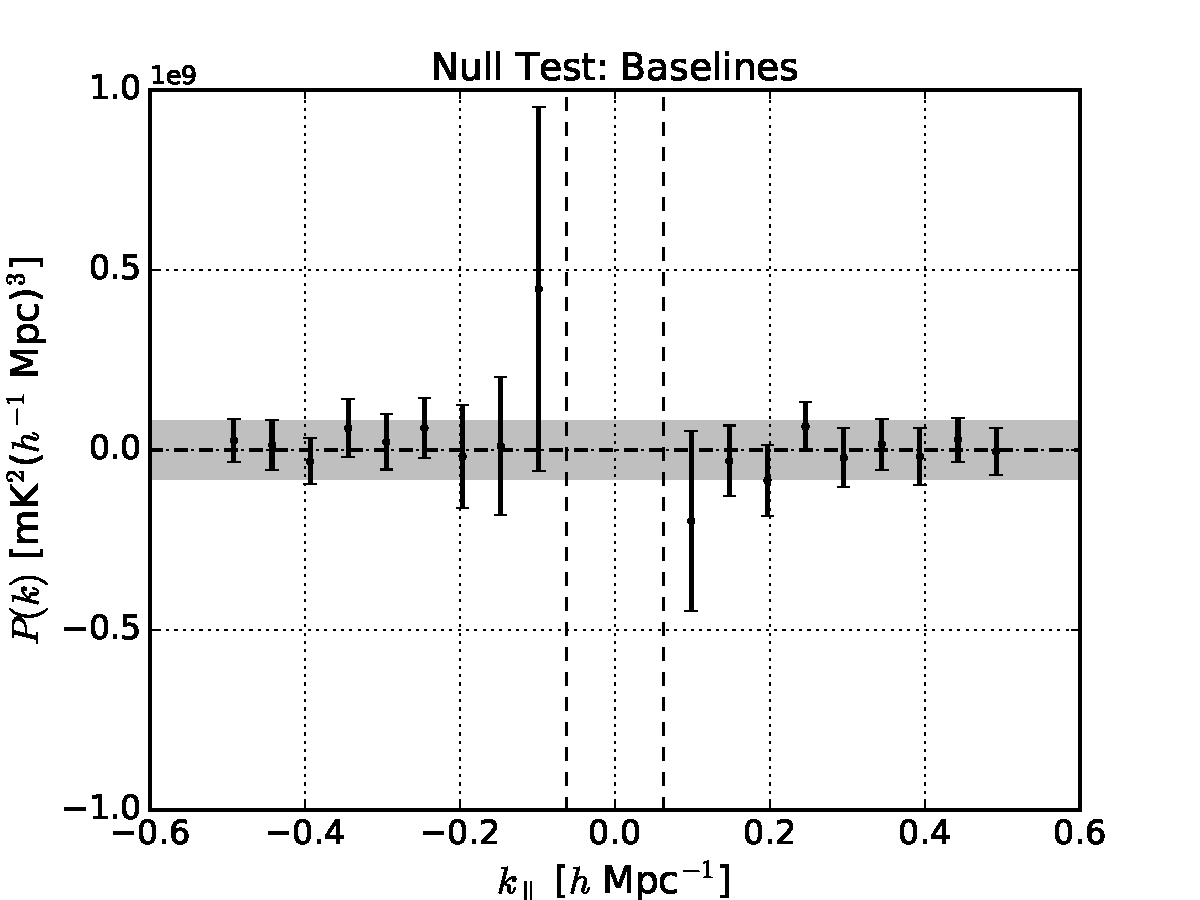
\includegraphics[width=0.47\textwidth]{plots/null_bls.pdf}
	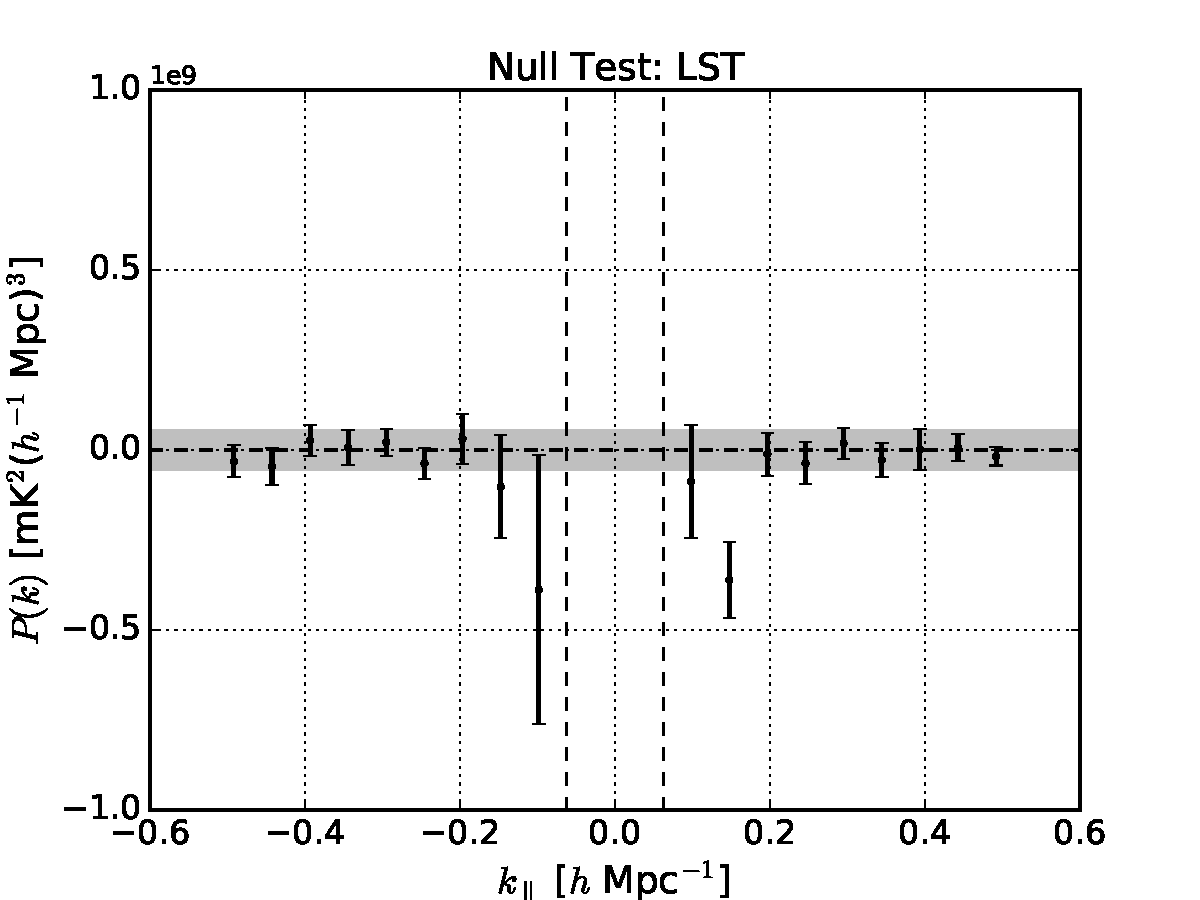
\includegraphics[width=0.47\textwidth]{plots/null_lsts.pdf}
	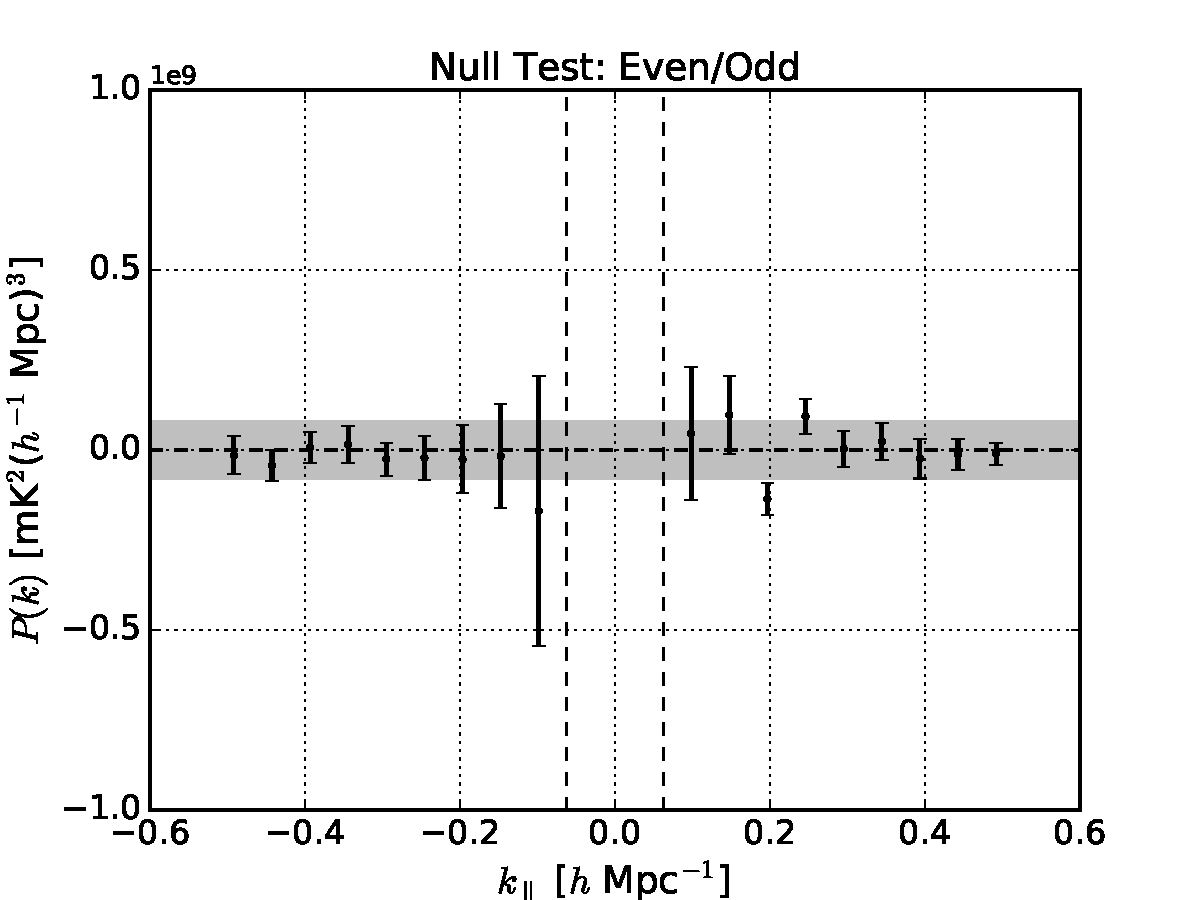
\includegraphics[width=0.47\textwidth]{plots/null_eo.pdf}
	\caption{Differenced power spectrum results (with $2\sigma$ bootstrapped errors) for three null tests, where a jackknife is taken along the baseline axis (top left), LST axis (top right), and even/odd Julian date axis (bottom). The results shown are unweighted (no signal loss), where the power spectrum values plotted are computed from the difference between two power spectra produced on either side of the jackknife axis. The gray shaded region in each plot is the estimated $2\sigma$ theoretical noise limit given the parameters of each test. We find that there are no significant systematics for $k > \pm 0.2$\,$h$ Mpc$^{-1}$ for all three tests. However, we find that all tests exhibit an extra variance at $k$-values near the horizon ($k\sim\pm 0.1$\,$h$ Mpc$^{-1}$), likely due to foreground-noise coupling terms when foregrounds are brightest. Additionally, we find that the LST null test is not fully consistent with zero, implying a bias that is LST dependent and likely caused by varying foregrounds.}
	\label{fig:null}
\end{figure*}

In investigating Figure \ref{fig:null}, we focus on three main possibilities --- whether the data points and error bars are consistent with thermal noise (``passing"), whether the error bars are consistent with zero but not consistent with thermal noise (``passing but has an additional variance"), or whether the error bars are not consistent with zero at all (``failing"). We examine each case in the context of our results below.

Firstly, all three null tests display data points that lie within the thermal noise gray band for $k > \pm 0.25$\,$h$ Mpc$^{-1}$. In addition, all three null tests show error bars consistent with the thermal noise level for those same $k$'s. This implies that the two jackknife halves do not differ by an amount greater than the thermal noise (i.e., the baselines making up the two jackknives either do not contain bias, or contain similar amounts of bias; we suspect it is the former though more thorough jackknives along this axis are needed to make this conclusion). We deem these as ``passing" null tests for the specific jackknives taken (again, dividing up the data in a different way along the same axes may not yield the same results, so more thorough testing is needed to be sure).

The second null test possibility (error bars consistent with zero but not with thermal noise) is displayed by the $k$-values just outside the horizon ($k\sim\pm 0.1$\,$h$ Mpc$^{-1}$) for all three tests. This indicates an additive noise component that is increasing our errors. More specifically, although we expect each cross-multiplication that is used in power spectrum estimation to have independent noise, there is still the possibility of a noise-foreground coupling term that can introduce power. This is because cross-multiplications produce four additive terms --- a signal-squared term (where ``signal" includes both foregrounds and EoR), two cross-terms between the signal and noise, and one noise-only term. When differencing two power spectra (each with their own four terms), we expect the signal-only term to subtract out for a ``passing" null test, and we expect the noise-only terms to be consistent with thermal noise. While the cross-terms have a mathematical expectation value of zero, in practice we are limited by our number of samples ($90$ cross-products for this analysis times $\sim$ $8$ independent LST samples). Combined with the fact that the foregrounds are so bright, the finite ensemble of the couplings can introduce extra variance that varies with foreground strength. It is therefore not surprising that this effect is largest at $k$-values just outside the horizon, where we expect foregrounds to be brightest post-delay filtering.

Lastly, a third null test result is an error bar not consistent with zero. This is the case for the LST null test at $k\sim-0.1$\,$h$ Mpc$^{-1}$ and $k\sim0.15$\,$h$ Mpc$^{-1}$, as well as the even/odd test at $k\sim0.2$\,$h$ Mpc$^{-1}$ and $k\sim0.25$\,$h$ Mpc$^{-1}$. In such a case, the two jackknife halves differ by an amount greater than the thermal noise (i.e., the data point is not in the thermal noise band), yet they are each constrained tightly by individual error bars that when combined, are not consistent with zero. This result implies that there exists a low level bias that is LST-dependent and Julian date-dependent. The former is likely caused by residual foregrounds that vary in LST, and it is not surprising that this type of bias occurs near the horizon limit. The latter requires further investigation that we leave to future work.

In this section we have presented the first jackknife and null tests from the PAPER experiment. Unsurprisingly, they imply that our measurements are biased by foregrounds, and not the EoR signal (a clean detection of EoR would have passed all three tests). While simple, these tests outline a framework that can be used by future measurements. The 21\,cm community is beginning to recognize the importance of these types of tests (\citealt{pober_et_al2016b}) in characterizing power spectra at the EoR level, and it is clear that future results will require more substantial and thorough investigations of this nature.

\section{Summary}

Although current 21\,cm published power spectrum upper limits lie several orders of magnitude above predicted EoR levels, 
ongoing analyses of deeper sensitivity datasets from PAPER, MWA, and LOFAR, as well as next generation instruments like 
HERA, are expected to continue to push towards EoR sensitivities. As the field progresses towards a detection, we have shown 
that it is crucial for future analyses to have a rigorous understanding of signal loss in an analysis pipeline and be able to accurately 
and robustly calculate both power spectrum and theoretical errors.

In particular, in Chapters \ref{c.PSmethods} and \ref{c.PSA64} we have investigated the subtleties and tradeoffs of common 21\,cm power spectrum techniques on 
signal loss and error estimation, which can be summarized as follows:

\begin{itemize}
\item Substantial signal loss can result when weighting data using empirically estimated covariances due to couplings with the data realizations (Chapter 
\ref{sec:SiglossOverview}). Loss of the 21\,cm signal is especially significant the fewer number of independent modes that
exist in the data. Hence, there exists a trade-off between sensitivity driven 
time-averaging techniques such as fringe-rate filtering and signal loss when using empirically estimated covariances. 
\item Signal injection and recovery simulations can be used to quantify signal loss (Chapter \ref{sec:siglossmethod}). However, a 
signal-only simulation (i.e., comparing a uniformly weighted vs. weighted power spectrum of EoR only) can underestimate loss by 
failing to account for correlations between the data and signal which can be large and negative.
\item Errors that are estimated via bootstrapping can be underestimated if samples in the dataset are significantly correlated 
(Chapter \ref{sec:Boot}). However, if the number of independent samples in a dataset is well-determined, bootstrapping is a 
simple and accurate way of estimating errors.
\end{itemize}

As a consequence of our investigations, we have also used a subset of PAPER-64 data to make a new power spectrum analysis. This serves as an illustrative example of using a signal injection framework, correctly computing errors via bootstrapping, and accurately estimating thermal noise. Our revised PAPER-64 limits are presented in Chapter \ref{c.PSA64_results}, which supersede all previously published PAPER limits. Because of the many challenges associated with signal loss and its estimation as described in this chapter, there we use a straightforward power spectrum estimation approach that is not lossy. However, the main reasons for a previously underestimated limit (\citealt{ali_et_al2018}) and 
ways in which our new analysis differs can still be summarized by the following:

\begin{itemize}
\item Signal loss, previously found to be $<2\%$ in \citetalias{ali_et_al2015}, was underestimated by a factor of $>$$1000$ for the case of empirically estimated inverse 
covariance weighting. Using a regularized covariance weighting method can minimize loss (Chapter 
\ref{sec:Weight}), however, because a regularized weighting method is not as aggressive as the former, it produces limits that are still higher than the lossy empirical inverse covariance limits. Underestimated signal loss therefore represents the bulk of our revision. 
\item Power spectrum errors, originally computed by bootstrapping, were underestimated for the data by a factor of $\sim2$ in mK due to oversampling data whose effective number of independent samples was reduced from fringe-rate filtering (Chapter \ref{sec:Boot}). Several other errors were also found regarding error estimation, though with smaller effects.
\item Several factors used in an analytic expression to predict the noise-level in PAPER-64 data were revised, yielding a 
decrease in predicted sensitivity level by a factor of $\sim3$ in mK (Chapter \ref{sec:Error}). We note that our sensitivity prediction is revised by a factor less than our overall
power spectrum result, implying that if taken at face value, the theoretical prediction for noise in \citetalias{ali_et_al2015} was too high for its data 
points.
\end{itemize}

The future of 21\,cm cosmology is exciting, as new experiments have sensitivities that expect to reach and surpass EoR levels, improved 
foreground mitigation and removal strategies are being developed, and simulations are being designed to better understand 
instruments. On the power spectrum analysis side, robust signal loss simulations and precise error calculations will play critical roles in accurate 21\,cm results. With strong foundations being established now, it is safe to say that we can expect to learn much about reionization and our early Universe in the coming years.

